%%%%%%%%%%%%%%%%%%%%%%%%%%%%%%%%%%%%%%%%%
% Short Sectioned Assignment LaTeX Template Version 1.0 (5/5/12)
% This template has been downloaded from: http://www.LaTeXTemplates.com
% Original author:  Frits Wenneker (http://www.howtotex.com)
% License: CC BY-NC-SA 3.0 (http://creativecommons.org/licenses/by-nc-sa/3.0/)
%%%%%%%%%%%%%%%%%%%%%%%%%%%%%%%%%%%%%%%%%

%----------------------------------------------------------------------------------------
%	PACKAGES AND OTHER DOCUMENT CONFIGURATIONS
%----------------------------------------------------------------------------------------

\documentclass[paper=a4, fontsize=11pt]{scrartcl} % A4 paper and 11pt font size

% ---- Entrada y salida de texto -----

\usepackage[T1]{fontenc} % Use 8-bit encoding that has 256 glyphs
\usepackage[utf8]{inputenc}
\usepackage{url}
%\usepackage{fourier} % Use the Adobe Utopia font for the document - comment this line to return to the LaTeX default

% ---- Idioma --------

\usepackage[spanish, es-tabla]{babel} % Selecciona el español para palabras introducidas automáticamente, p.ej. "septiembre" en la fecha y especifica que se use la palabra Tabla en vez de Cuadro

% NOTA: en caso de problema al compilar, compruebe que tiene el paquete: texlive-babel-spanish.noarch

% ---- Otros paquetes ----

\usepackage{amsmath,amsfonts,amsthm} % Math packages
\usepackage{graphics,graphicx,floatrow} %para incluir imágenes y notas en las imágenes
\usepackage{listings}


% Para hacer tablas comlejas
\usepackage{multirow}
\usepackage{threeparttable}

%\usepackage{sectsty} % Allows customizing section commands
%\allsectionsfont{\centering \normalfont\scshape} % Make all sections centered, the default font and small caps

\usepackage{fancyhdr} % Custom headers and footers
\pagestyle{fancyplain} % Makes all pages in the document conform to the custom headers and footers
\fancyhead{} % No page header - if you want one, create it in the same way as the footers below
\fancyfoot[L]{} % Empty left footer
\fancyfoot[C]{} % Empty center footer
\fancyfoot[R]{\thepage} % Page numbering for right footer
\renewcommand{\headrulewidth}{0pt} % Remove header underlines
\renewcommand{\footrulewidth}{0pt} % Remove footer underlines
\setlength{\headheight}{13.6pt} % Customize the height of the header

\numberwithin{equation}{section} % Number equations within sections (i.e. 1.1, 1.2, 2.1, 2.2 instead of 1, 2, 3, 4)
\numberwithin{figure}{section} % Number figures within sections (i.e. 1.1, 1.2, 2.1, 2.2 instead of 1, 2, 3, 4)
\numberwithin{table}{section} % Number tables within sections (i.e. 1.1, 1.2, 2.1, 2.2 instead of 1, 2, 3, 4)

\setlength\parindent{0pt} % Removes all indentation from paragraphs - comment this line for an assignment with lots of text

\newcommand{\horrule}[1]{\rule{\linewidth}{#1}} % Create horizontal rule command with 1 argument of height


%----------------------------------------------------------------------------------------
%	TÍTULO Y DATOS DEL ALUMNO
%----------------------------------------------------------------------------------------

\title{	
\normalfont \normalsize 
\textsc{{\bf Sistemas Multimedia (2014-2015)} \\ Grado en Ingeniería Informática \\ Universidad de Granada} \\ [25pt] % Your university, school and/or department name(s)
\horrule{0.5pt} \\[0.4cm] % Thin top horizontal rule
\huge Memoria Práctica Final  \\ % The assignment title
\horrule{2pt} \\[0.5cm] % Thick bottom horizontal rule
}

\author{Francisco Javier Garrido Mellado} % Nombre y apellidos

\date{\normalsize\today} % Incluye la fecha actual

%----------------------------------------------------------------------------------------
% DOCUMENTO
%----------------------------------------------------------------------------------------

\begin{document}

\maketitle % Muestra el Título

\newpage %inserta un salto de página

\tableofcontents % para generar el índice de contenidos

\listoffigures

%\listoftables

\newpage
%----------------------------------------------------------------------------------------
%	Introducció
%----------------------------------------------------------------------------------------
\section{Introducción }
En el presente documento se explican los pasos seguidos para la elaboración de la práctica Final de Sistemas Multimedia. Esta práctica consiste en dar continuidad a las practicas anteriores añadiendole mas funcionalidad, para ello es necesario la elaboración de clases propias.
La aplicación cuenta con un entorno multiventa siendo \emph{VentanaPrincipal} la ventana que cuenta con las diferentes barras de herramientas.
\textbf{Nota: El proyecto UML se ha realizado con Netbeans.}
%-----------------------------------------------------------------
%--------------------------------------------------
\section{Funcionalidad y manejo de la interfaz }
En este apartado se explica la funcionalidad y uso de cada barra de herramientas de la interfaz.
\subsection{Menú Archivo}
En este menú se encuentra las siguientes opciones en orden respectivo:
\begin{itemize}
\item \textbf{Nuevo} -Abre un nuevo lienzo con el tamaño especificado.
\item \textbf{Abrir} -Abre una imagen, video o audio.
\item \textbf{Guardar} - Guarda la imagen en el formato especificado\cite{guardar}.
\item \textbf{Abrir Audio} -Abre archivo de audio con formato wav, au o aif.Usa Java Sound API.
\item \textbf{Guardar Audio} -Guarda archivo de audio.Primero se introduce nombre del archivo y despues se lanza VentanaInternaGrabador. 
\item \textbf{Ventana Reproduccion} -Usa JMF API y permite abrir archivos de audio y video.
\item \textbf{Ventana Camara} - Usa tambien JMF API y permite visualizar lo que recoge la webcam.
\item \textbf{Ventana Captura} - Realiza captura de lo que muestra la webcam o la ventana de reproducción. 
\end{itemize}


\begin{figure}[H]
  \centering
    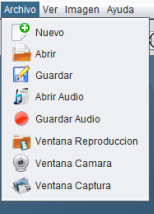
\includegraphics[scale=0.70]{images/menuarchivofinal}
  \caption{Menu Archivo}
  \label{Menu Archivo}
\end{figure}

\subsection{Menú Ver}
En este menú hay cuatro opciones de visualización:
\begin{itemize}
\item \textbf{Barra de estados} -Muestra/oculta los textlabel que indican la selección de la forma,de borde y relleno.
\item \textbf{Barra de formas} -Muestra/oculta los botones para seleccionar forma geométrica y editar.
\item \textbf{Barra de atributos} - Muestra/oculta la barra para especificar color, grosor,alisado,etc.
\item \textbf{Barra de atrib. de imagen} -Muestra/oculta la barra de herramientas de imágenes.
\end{itemize}

\subsection{Menú Imagen}
En este menú se encuentra las siguientes opciones en orden respectivo:
\begin{itemize}
\item \textbf{RescaleOp} -A cada componente de un pixel le realiza una transformación.
\item \textbf{ConvolveOp} -Aplica mascara de convolución.
\item \textbf{AffineTransformOp} - Realiza una transformación afín.
\item \textbf{LookupOp} -Realiza una transformacion T sobre los niveles de color.
\item \textbf{BandCombineOp} -Realiza una combinación lineal de las bandas de una imagen. 
\item \textbf{ColorConvertOp} -Realiza una conversión del espacio de color pixel a pixel.
\item \textbf{Duplicar} - Realiza un duplicado de una imagen.
\item \textbf{Negativo} - Realiza negativo de una imagen. 
\item \textbf{ConversionGris} -Transforma una imagen en color a escala de grises.
\item \textbf{TintadoOp} -Realiza un tintado de la imagen segun el color seleccionado en la paleta de colores.
\item \textbf{Transf.Logaritmo} -Aplica operación de transformacion logaritmica a una imagen.
\item \textbf{Raiz n-esima} - Aplica operación de transformacion raiz n-esima a una imagen.
\item \textbf{Potencia n-esima} - Aplica operación de transformacion de potencia n-esima a una imagen. 
\item \textbf{EliminarMitadBandaCentral} -Se reduce la banda central de RGB a la mitad.
\end{itemize}


\begin{figure}[H]
  \centering
    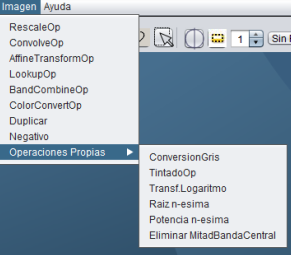
\includegraphics[scale=0.70]{images/menuimagenfinal}
  \caption{Menu Imagen}
  \label{Menu Imagen}
\end{figure}

\subsection{Menú Ayuda}
En este menú se encuentra la siguiente opción:

\begin{itemize}
\item \textbf{Acerca de} -Muestra autor, nombre del programa y su version
\end{itemize}

\subsection{Barra archivo}
En este menú se encuentra las siguientes opciones en orden respectivo( cumplen la misma función que en menu archivo) :
\begin{itemize}
\item \textbf{Nuevo} .
\item \textbf{Abrir} 
\item \textbf{Guardar} .

\end{itemize}
\begin{figure}[H]
  \centering
    
\includegraphics[scale=0.80]{images/barraarchivo}
  \caption{Barra Archivo}
  \label{Barra Archivo}
\end{figure}


\subsection{Barra de formas}
En este menú se encuentra las siguientes opciones en orden respectivo:
\begin{itemize}
\item \textbf{Punto} -Selección del punto como forma geométrica.
\item \textbf{Linea} -Selección de la linea como forma geométrica.
\item \textbf{Rectángulo} -Selección del rectangulo como forma geométrica.
\item \textbf{Elipse} -Selección de la elipse como forma geométrica.
\item \textbf{Rectángulo Redondeado} -Selección del rectángulo redondeado como forma geométrica. 
\item \textbf{Curva} -Selección de la curva como forma geométrica.
\item \textbf{Editar} - Selección de editado de las formas geométricas, al seleccionar esta opción posteriormente se selecciona los atributos deseados y por último la figura a la que se le aplicará, pudiendose mover a otra posición del lienzo tambien.

\end{itemize}


\begin{figure}[H]
  \centering
    
\includegraphics[scale=0.80]{images/barraformas}
  \caption{Barra Formas}
  \label{Barra Formas}
\end{figure}


\subsection{Barra de atributos}
En este menú se encuentra las siguientes opciones en orden respectivo:
\begin{itemize}
\item \textbf{Alisado} -Selección del modo alisado al dibujar la figura geométrica.
\item \textbf{Discontinuidad} -Establece el trazo como discontinuo.
\item \textbf{Grosor} -Establece el grosor del trazo.
\item \textbf{Relleno} -Establece tipo de relleno solido, degradado horizontal, degradado vertical o sin relleno.
\item \textbf{Transparencia} -Establece transparencia de un 25, 50 o 75 por ciento o sin transparencia. 
\item \textbf{Color} -Permite elegir color, se permite elegir entre una paleta de colores.

\end{itemize}


\begin{figure}[H]
  \centering
    
\includegraphics[scale=0.80]{images/barraatributos}
  \caption{Barra Atributos}
  \label{Barra Atributos}
\end{figure}

\subsection{Barra Multimedia}
En este menú se encuentra las siguientes opciones en orden respectivo:
\begin{itemize}
\item \textbf{Abrir Multimedia} -Permite abrir archivo de audio o video.
\item \textbf{WebCam} -Permite visualizar en pantalla lo que recoge la webcam.
\item \textbf{Capturar} -Captura instantanea del reproductor multimedia o de la webcam.
\item \textbf{Grabar audio} -Permite grabar audio al igual que se explicó en el menu Archivo.
\item \textbf{Abrir Multimedia con Barra de Progreso} -Permite reproducir archivo de audio adjuntandose una barra de progreso.
\item \textbf{Reproductor de Audio con Barra de Progreso} -Misma funcionalidad que antes pero sin lanzar una ventana, esta se desarrolla en la VentanaPrincipal.
\end{itemize}


\begin{figure}[H]
  \centering
    
\includegraphics[scale=0.80]{images/barra_multimedia}
  \caption{Barra Multimedia}
  \label{Barra Multimedia}
\end{figure}



\subsection{Barra de Atributos de Imagen}
En este menú se encuentra las siguientes opciones en orden respectivo:
\begin{itemize}
\item \textbf{Brillo} -Permite modificar el brillo de una imagen con un deslizador.
\item \textbf{Filtro} -Permite aplicar un filtro a la imagen entre un abanico de cinco posiblidades( Media, Binomial, Enfoque, Relieve y Frontera Laplaciana).
\item \textbf{Contraste} -Permite las opcines de dar contraste, iluminar u oscurecer una imagen.
\item \textbf{Seno} -Aplica filtro seno a una imagen.
\item \textbf{Rotación}- Permite rotar una imagen usando un deslizador o botones con rotaciones fijas de 90,180 o 270 grados.
\item \textbf{Escala}- Permite escalar una imagen usando un factor de 1.25 (aumentar) o 0.75 (disminuir).

\item \textbf{Umbralizacion Color y Gris}- Permite umbralizar una imagen a escala de grises o al color seleccionado en la paleta de colores.
\item \textbf{Binarias}- Realiza las operaciones de Blending para mezclar imágenes o de resta para establecer diferencias.
\end{itemize}

\begin{figure}[H]
  \centering
    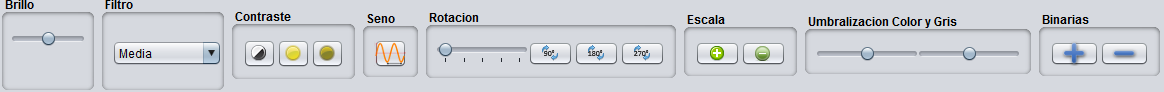
\includegraphics[scale=0.40]{images/barraatributosimagen}
  \caption{Barra Atributo Imagen}
  \label{Barra Atributo Imagen}
\end{figure}

%----------------------------------------------------------------------------------------
%	Cuesti´on 1
%----------------------------------------------------------------------------------------
\section{Entorno multiventana. }
Se ha procedido a usar una Ventana Principal como principal interfaz de la practica,dicha clase \emph{VentanaPrincipal} hereda de \emph{JFrame} y contiene las barras de herramientas para asignar forma geométrica, atributos a las formas geométricas, efectuar operaciones sobre imágenes, y las relativas a la apertura de audio y video.
\begin{figure}[H]
  \centering
    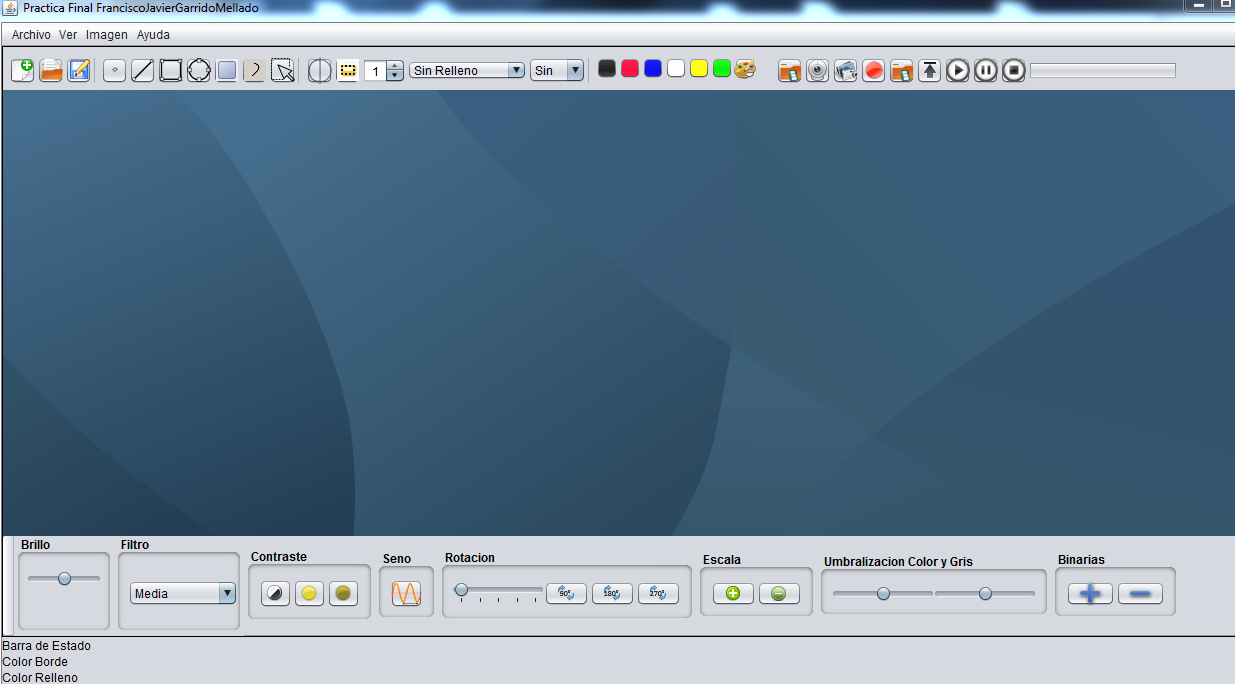
\includegraphics[scale=0.45]{images/interfaz_}
  \caption{Interfaz}
  \label{Interfaz}
\end{figure}
Al efectuar una apertura de imagen o bien abrir un nuevo lienzo se lanza la ventana de imagen que no es otra cosa que la clase \textbf{VentanaInterna} que 'contiene' la clase \textbf{Lienzo2DImagenfinal} y es donde se pinta y se realizan las operaciones de imágenes.
Por otra parte, se dispone de otras cuatro ventanas que son usadas para todo lo relacionado con audio o video:
\begin{itemize}
\item \textbf{VentanaInternaCamara} - Ventana que muestra lo que recoge la webcam.
\item \textbf{VentanaInternaGrabador} - Ventana para grabar audio.
\item \textbf{VentanaInternaJMFPlayer} - Ventana para reproducir audio o video.
\item \textbf{VentanaInternaReproductor} - Ventana para reproducir audio.
\item \textbf{VentanaInternaReproductorHebra} - Ventana para reproducir audio con el añadido de una barra de progreso lanzada con una hebra.

\end{itemize}
\begin{figure}[H]
  \centering
    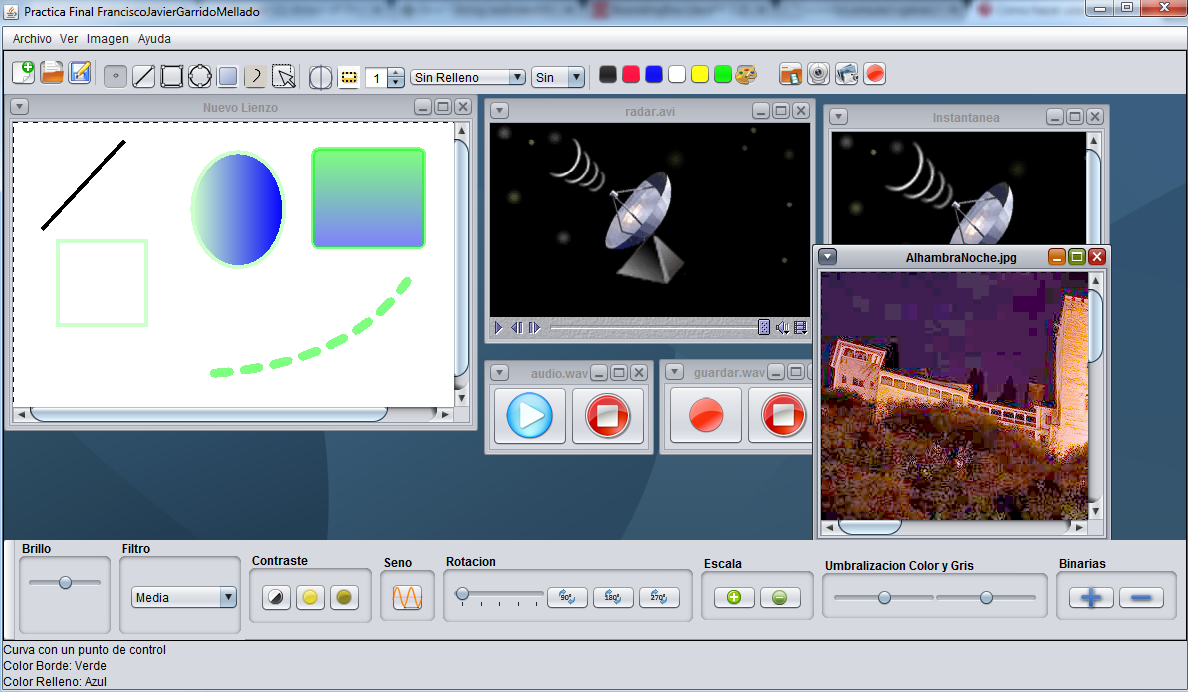
\includegraphics[scale=0.40]{images/interfaz_con_ventanas}
  \caption{Interfaz con todas las ventanas}
  \label{Interfaz con todas las ventanas}
\end{figure}
\subsection{Ventana Principal}

Como se ha comentado esta ventana recoge las barras de herramientas para seleccionar la forma geómetrica con la que se dibuja, sus atributos como grosor, tipo de transparencia, alisado, etc, operaciones de imágenes como rotar, umbralización por color o niveles de gris, abrir un nuevo video, etc.Además se dispone de cuatro menus:
\begin{itemize}
\item \textbf{Archivo}- Para abrir un lienzo nuevo, una nueva imagen, el reproductor de audio, grabar audio, una nueva reproducción multimedia o la webcam.
\item  \textbf{Ver}- Para dejar a la vista las diferentes barras de herramientas y los textlabel.
\item \textbf{Imagen}- Recoge diferentes operaciones sobre imágenes incluyendo las de cosecha propia.
\item \textbf{Info}-Muestra mi nombre y la versión de la práctica.
\end{itemize} 
\begin{figure}[H]
  \centering
    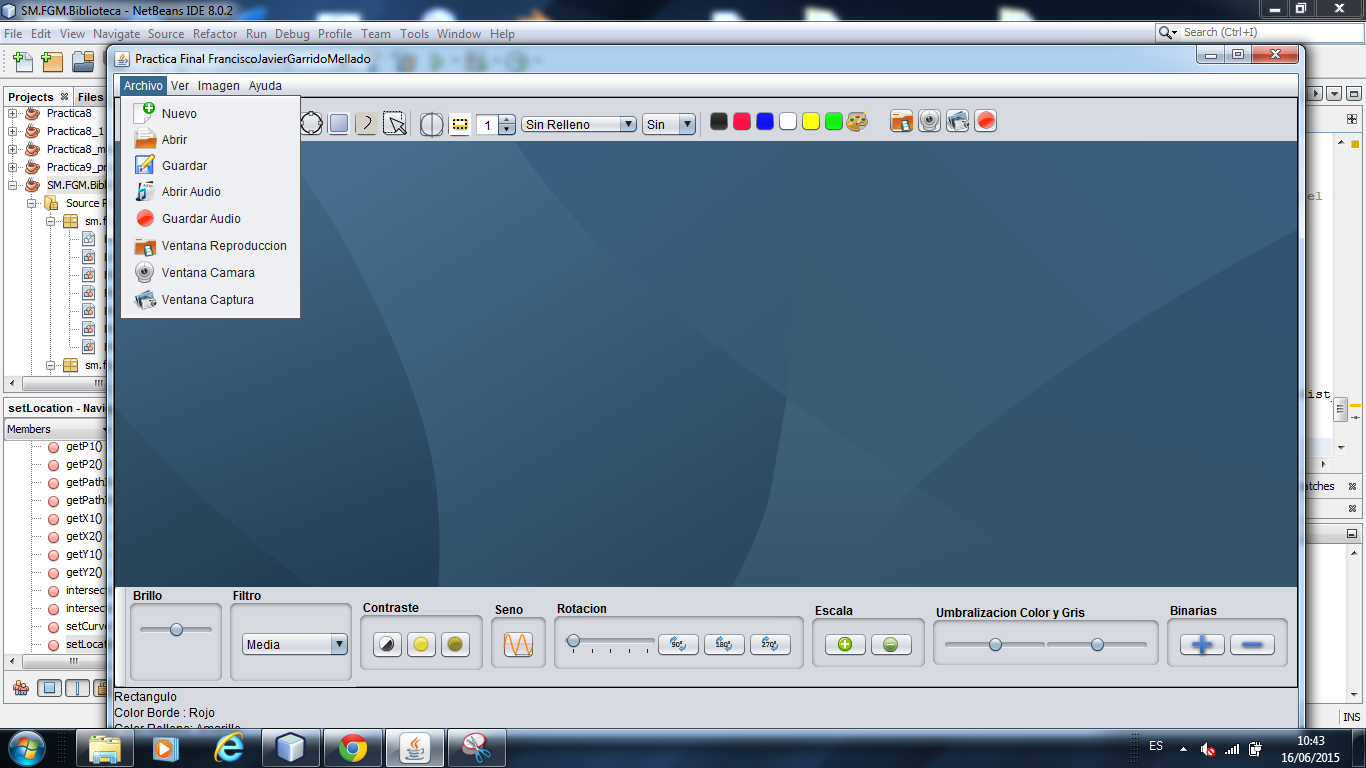
\includegraphics[scale=0.40]{images/menuarchivo}
  \caption{Menu de Archivo}
  \label{Menu de Archivo}
\end{figure}
\begin{figure}[H]
  \centering
    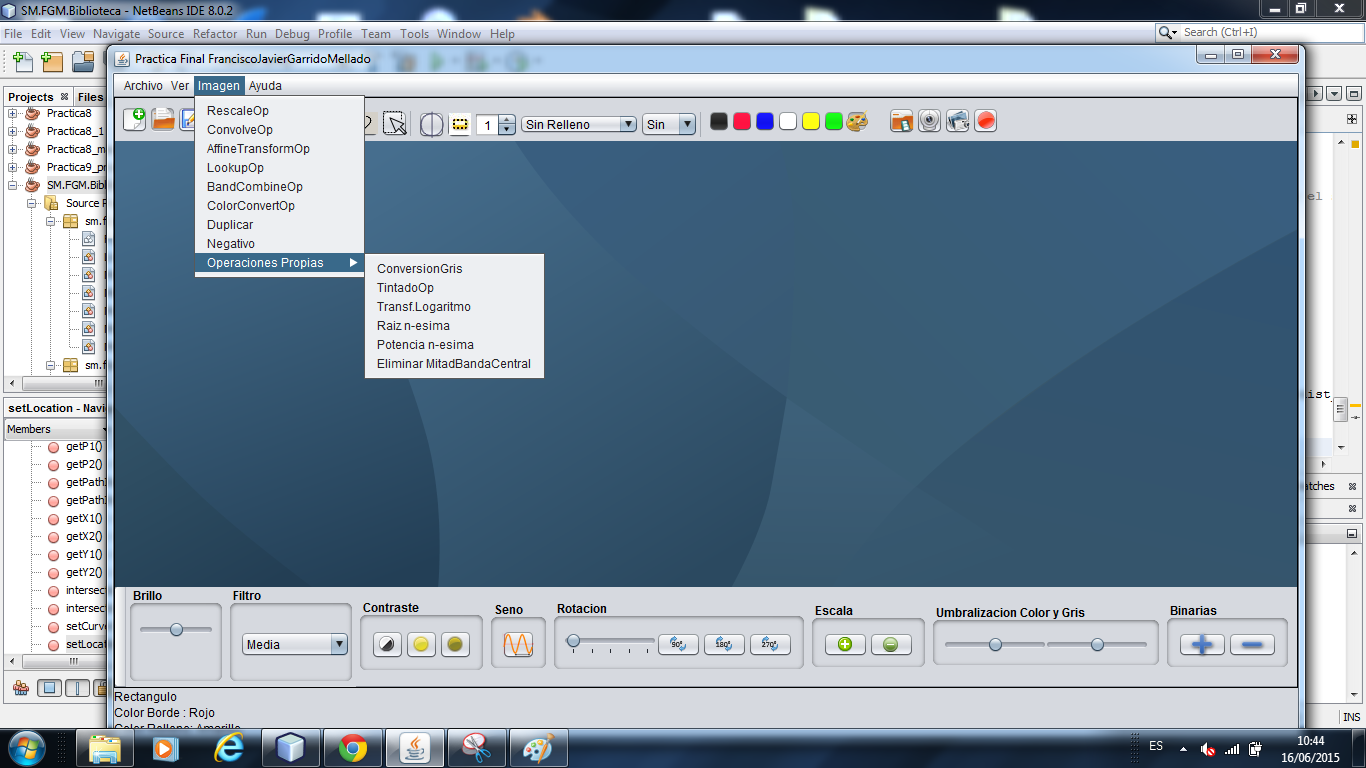
\includegraphics[scale=0.40]{images/menuimagen}
  \caption{Menu de Imagen}
  \label{Menu de Imagen}
\end{figure}

Realmente lo que hace esta y el resto de ventanas es recoger un evento y efectuar la operación correspondiente ( usando el objeto lienzo correspondiente que es donde se carga el dibujo o imagen).Para su diseño se ha heredado de \emph{javax.swing.JFrame}.(Nota:Debido a lo amplio que es el UML de VentanaPrincipal se recomienda abrir el proyecto UML con Netbeans o la imagen que esta alojada en la carpeta images de Latex\_Final).
\begin{figure}[H]
  \centering
    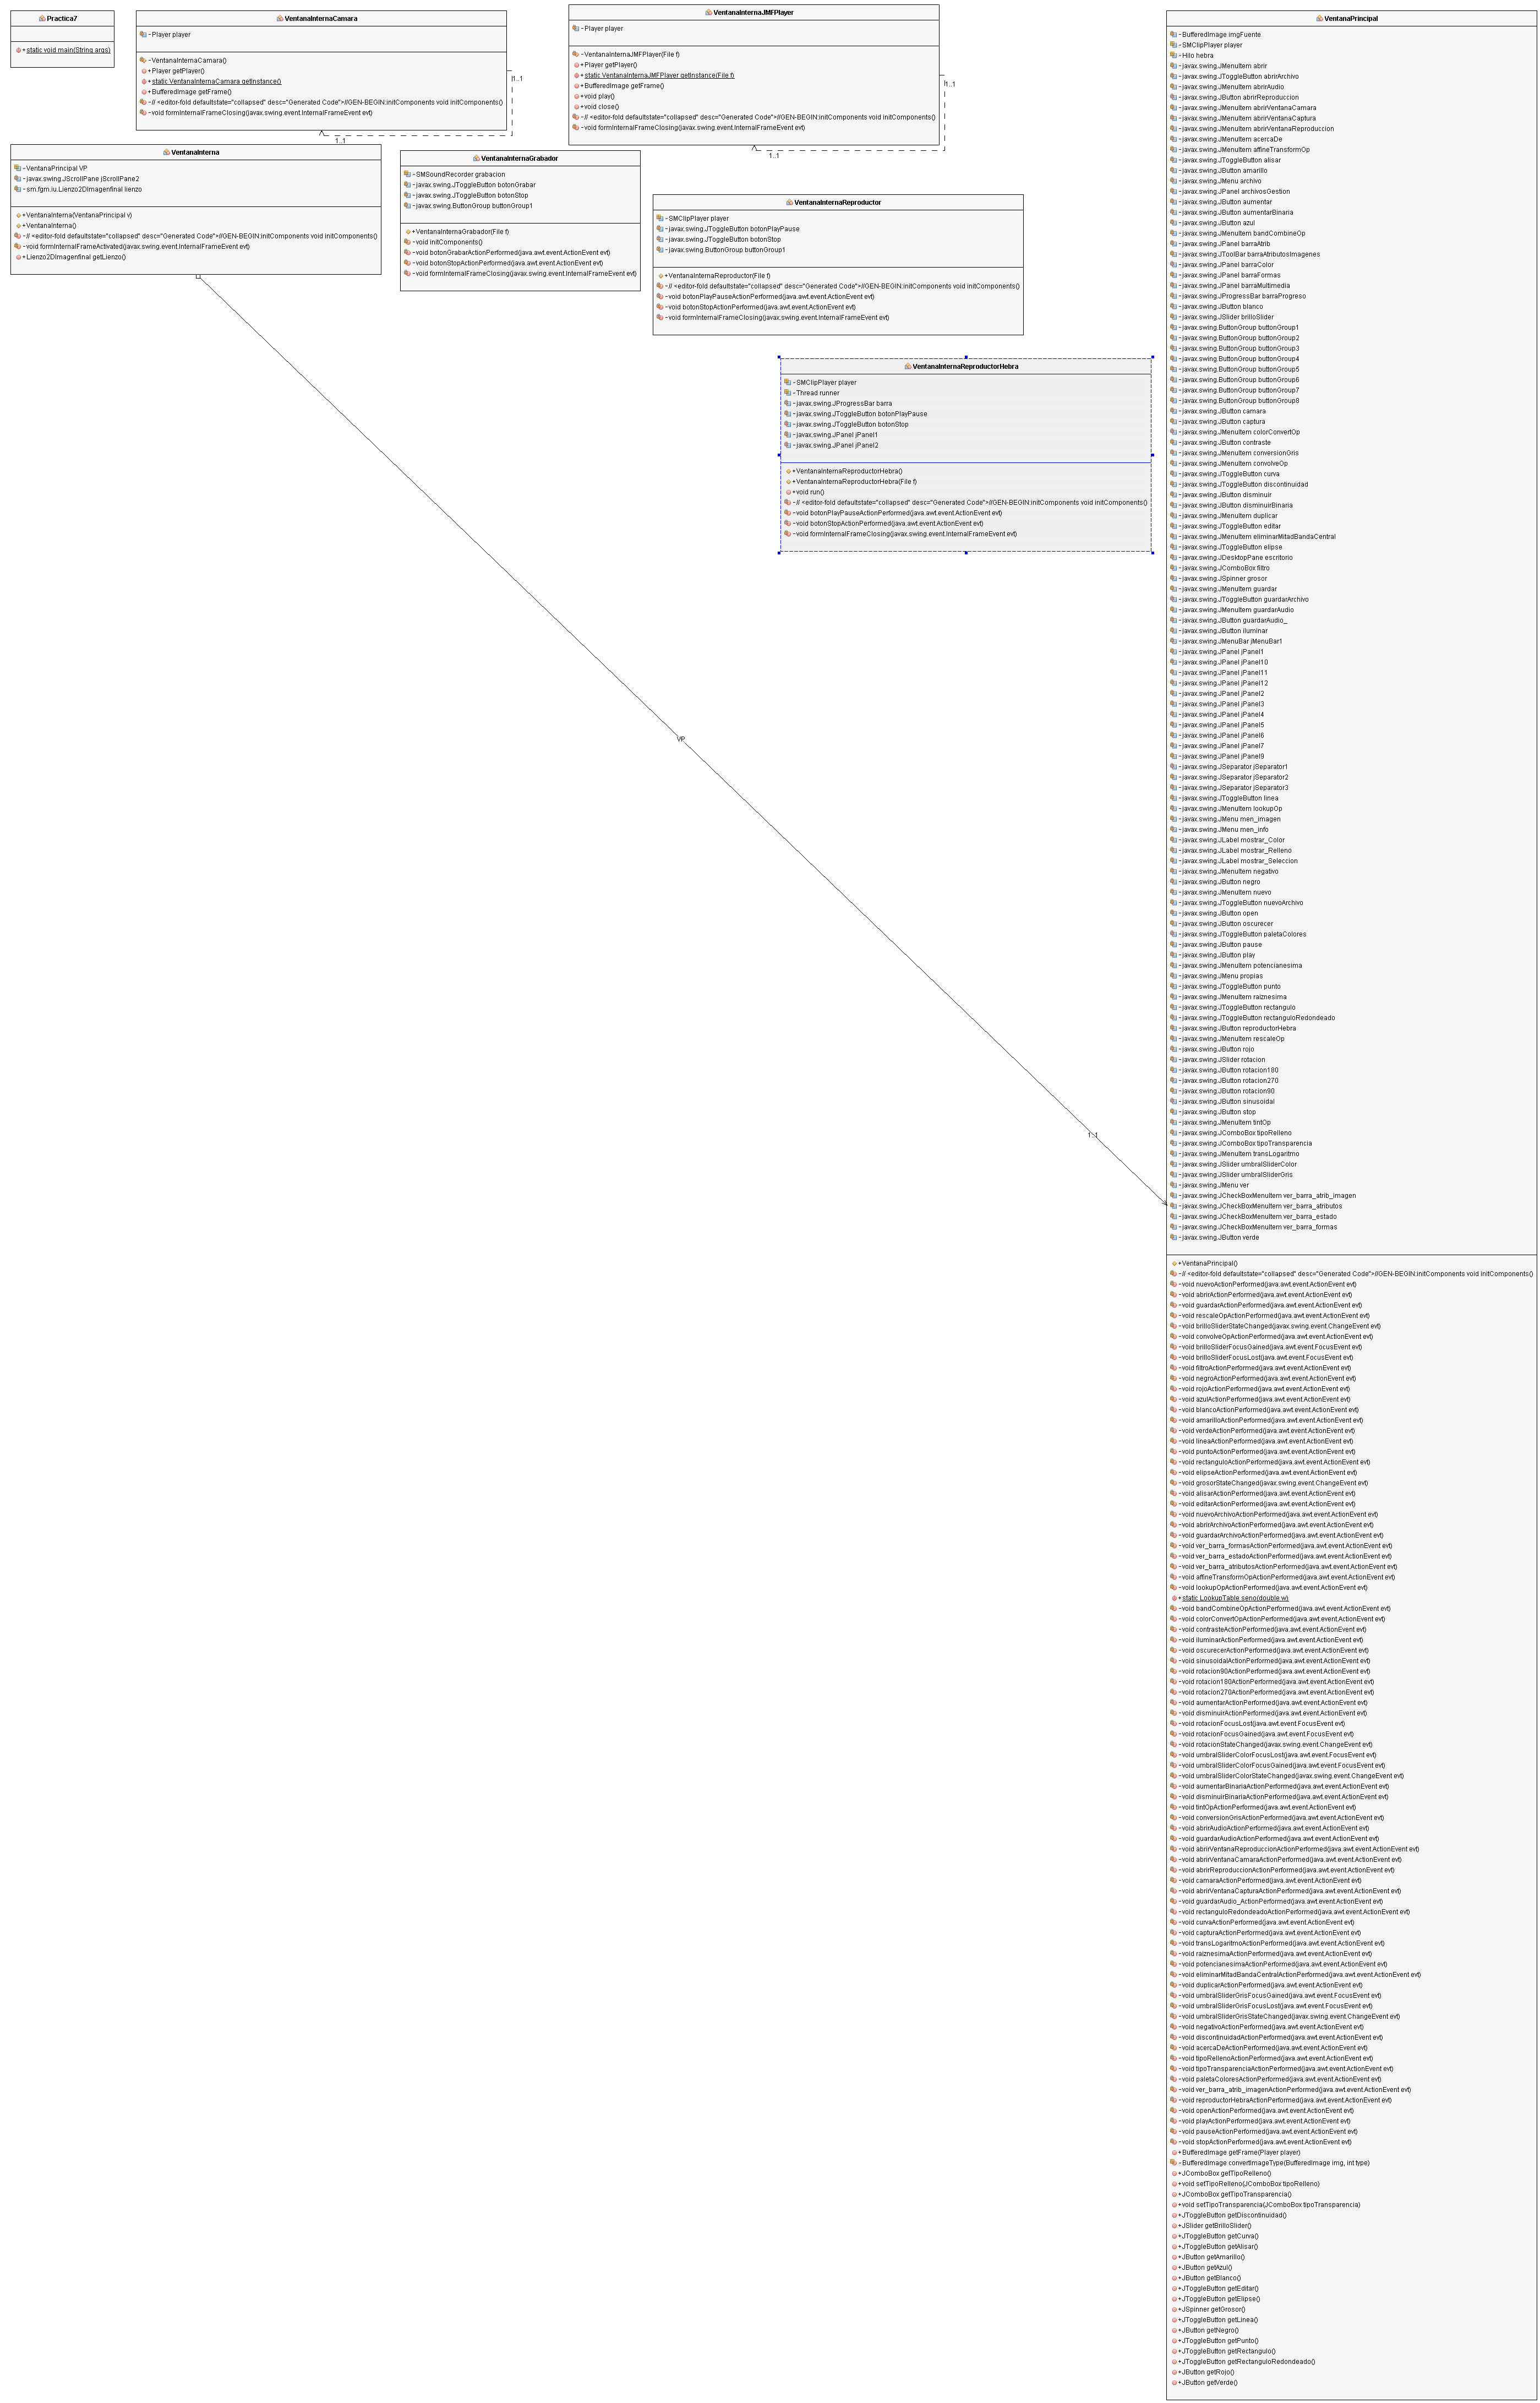
\includegraphics[scale=0.10]{images/Ventanas}
  \caption{UML Ventanas}
  \label{UML Ventanas}
\end{figure}



De los métodos de Ventana Principal destaco los siguientes:
\begin{itemize}
\item \textbf{ private void nuevoArchivoActionPerformed(java.awt.event.ActionEvent evt)}- Para abrir un lienzo nuevo con el tamaño especificado.
\item  \textbf{private void abrirArchivoActionPerformed(java.awt.event.ActionEvent evt)}- Para abrir un fichero, segun la extensión se abre una ventana u otra.
\item \textbf{private void tintOpActionPerformed(java.awt.event.ActionEvent evt)}- Realiza un tintado de la imagen segun el color seleccionado en la paleta de colores, se usa clase propia para realizar la operación.
\item \textbf{private void conversionGrisActionPerformed(java.awt.event.ActionEvent evt)}-Convierte a niveles de gris una imagen usando unos factores de conversión.Usa clase propia.
\item \textbf{private void abrirVentanaCapturaActionPerformed(java.awt.event.ActionEvent evt)}- Realiza una captura de pantalla del video o de la webcam.
\item \textbf{private void raiznesimaActionPerformed(java.awt.event.ActionEvent evt)}- Aplica una operación de raiz nesima a una imagen, se ha usado clase propia, ademas se dispone de otras operaciones similares.
\end{itemize} 
Pueden comentarse muchos mas como la umbralizacion por escala de grises donde se usa una clase propia, la paleta de colores, etc.
\begin{lstlisting}
private void nuevoArchivoActionPerformed(java.awt.event.ActionEvent evt) {
        VentanaInterna vi = new VentanaInterna(this);
        
        JTextField ancho= new JTextField("300");
        JTextField alto= new JTextField("300");
        JFileChooser dlg = new JFileChooser();        

        Object[] ancho_alto ={ "Ancho ",ancho,"Alto",alto };
        JOptionPane.showConfirmDialog(this, ancho_alto,"Introduzca 
        anchura y altura",JOptionPane.DEFAULT_OPTION);
                       
        
        escritorio.add(vi);
        vi.setVisible(true);
        BufferedImage img;
        img = new BufferedImage(Integer.parseInt(ancho.getText()),
        Integer.parseInt(alto.getText()),BufferedImage.TYPE_INT_RGB);

        img.createGraphics().setPaint(Color.WHITE);//permite pintar en el
        img.createGraphics().fill(new Rectangle2D.Float(0,0,img.getWidth(),
        img.getHeight()));
        Lienzo2DImagenfinal li= (Lienzo2DImagenfinal)vi.getLienzo();
        li.setImage(img);
        }
\end{lstlisting}    
\begin{lstlisting}
 private void abrirArchivoActionPerformed(java.awt.event.ActionEvent evt) {
JFileChooser dlg = new JFileChooser();
        FileNameExtensionFilter filter = new 
        FileNameExtensionFilter("Imagenes", ImageIO.getWriterFormatNames());
      
        dlg.addChoosableFileFilter(filter);
        
        String extension[]={"wav","mp3","ogg","avi","mpg"};  
        FileNameExtensionFilter filtro = new 
        FileNameExtensionFilter("Videos y Audio",extension);
        dlg.addChoosableFileFilter(filtro);
       
        dlg.setFileFilter(filter);
        dlg.setFileFilter(filtro);
        dlg.setAcceptAllFileFilterUsed(false);
        
        
            int resp = dlg.showOpenDialog(this);
            if( resp == JFileChooser.APPROVE_OPTION) {
                
                File f = dlg.getSelectedFile();
                
                if(dlg.getFileFilter()==filter){
                    try{
                      BufferedImage img = ImageIO.read(f);
                      VentanaInterna vi = new VentanaInterna(this);
                      vi.getLienzo().setImage(img);
                      this.escritorio.add(vi);
                      vi.setTitle(f.getName());
                      vi.setVisible(true);
                    } catch(Exception ex){ 
                    System.err.println("Error al leer la imagen");
                     }
                  }else if(dlg.getFileFilter()==filtro){
                      try{
                    JInternalFrame vi = 
                    VentanaInternaJMFPlayer.getInstance(f);
                    this.escritorio.add(vi);
                    vi.setTitle(f.getName());
                    vi.setVisible(true);
                      }catch(Exception ex){ 
                      System.err.println("Error al abrir video");
                     }
                }
                

}
    }
\end{lstlisting}
\begin{lstlisting}
private void tintOpActionPerformed(java.awt.event.ActionEvent evt) {
        JInternalFrame vi = escritorio.getSelectedFrame();
        if ((vi != null)&&(vi instanceof VentanaInterna)) {
            BufferedImage imgSource = 
            ((VentanaInterna)vi).getLienzo().getImage();
        if(imgSource!=null){
            
        try{
            
            TintadoOp top= new TintadoOp(
            ((VentanaInterna)vi).getLienzo().getColor(),0.5F);
            
            BufferedImage imgdest = top.filter(imgSource, null);
            ((VentanaInterna)vi).getLienzo().setImage(imgdest);
            ((VentanaInterna)vi).getLienzo().repaint();
          }catch(IllegalArgumentException e){
           System.err.println(e.getLocalizedMessage());
          }
        }
        } 
    }
\end{lstlisting}
\begin{lstlisting}
private void conversionGrisActionPerformed(java.awt.event.ActionEvent 
evt) {
        JInternalFrame vi = escritorio.getSelectedFrame();
        if ((vi != null)&&(vi instanceof VentanaInterna)) {
            BufferedImage imgSource = 
            ((VentanaInterna)vi).getLienzo().getImage();
        if(imgSource!=null){
           
            try{
              ConversionGrisOp gop = new ConversionGrisOp();
            
            BufferedImage imgdest = gop.filter(imgSource, null);
            ((VentanaInterna)vi).getLienzo().setImage(imgdest);
            ((VentanaInterna)vi).getLienzo().repaint();
        } catch(IllegalArgumentException e){
            System.err.println(e.getLocalizedMessage());
}
}
}
\end{lstlisting}
\begin{lstlisting}
 private void abrirVentanaCapturaActionPerformed(
                   java.awt.event.ActionEvent evt) {
        VentanaInterna vi= new VentanaInterna(this);
        JInternalFrame vic = escritorio.getSelectedFrame();
        if(vic instanceof VentanaInternaCamara){
          try{
            vi.getLienzo().setImage(this.getFrame(
            ((VentanaInternaCamara)vic).getPlayer()));
            vi.setTitle("Instantanea");
            vi.setLocation(20+vi.getWidth(),0);
            vi.setVisible(true);
            this.escritorio.add(vi);
            }
          catch (Exception ex)
           {
        System.err.println("Error 1");
           }
        }else if(vic instanceof VentanaInternaJMFPlayer){
            try{
            vi.getLienzo().setImage(getFrame(
            ((VentanaInternaJMFPlayer)vic).getPlayer()));
           // vi.getLienzo().setImage(
           ((VentanaInternaJMFPlayer)vic).getFrame());  
            vi.setTitle("Instantanea");
            vi.setLocation(20+vi.getWidth(),0);
            vi.setVisible(true);
            this.escritorio.add(vi);
            }
          catch (Exception ex)
          {
        System.err.println("Error");
      }
        }
    
\end{lstlisting}
\begin{lstlisting}
private void raiznesimaActionPerformed(java.awt.event.ActionEvent evt) {
   JInternalFrame vi = escritorio.getSelectedFrame();

   if ((vi != null)&&(vi instanceof VentanaInterna)) {
     BufferedImage imgSource = 
     ((VentanaInterna)vi).getLienzo().getImage();
     if(imgSource!=null){
       try{
         JTextField raz= new JTextField("2");
         JFileChooser dlg = new JFileChooser();        

         Object[] v_raz ={ "Raiz n-esima ",raz };
         JOptionPane.showConfirmDialog(this, v_raz,
         "Introduzca valor Raiz n-esima",JOptionPane.DEFAULT_OPTION);

         LookupTable lt =RaizNesima.raiz(
         Double.parseDouble(raz.getText()));
                 
         LookupOp lop = new LookupOp(lt, null);
        // Imagen origen y destino iguales
        lop.filter( imgSource , imgSource);
        vi.repaint();
                    
      } catch(Exception e){
        System.err.println(e.getLocalizedMessage());
        }
            }
    }


\end{lstlisting}


\subsection{VentanaInterna}
Esta clase es la ventana que se abre para dibujar o bien sobre un lienzo o sobre una imagen que se carga.
\begin{figure}[H]
  \centering
    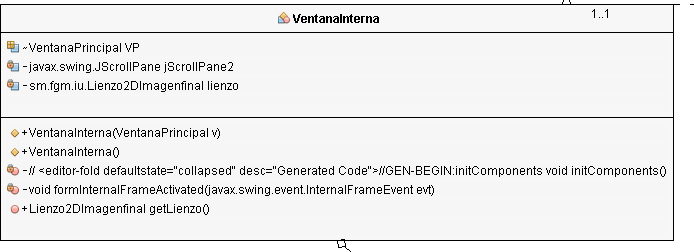
\includegraphics[scale=0.60]{images/ventanaInterna}
  \caption{UML VentanaInterna}
  \label{UML VentanaInterna}
\end{figure}
\begin{lstlisting}
 private void initComponents() {

        jScrollPane2 = new javax.swing.JScrollPane();
        lienzo = new sm.fgm.iu.Lienzo2DImagenfinal();
        ...
        }
\end{lstlisting}
Se ha diseñado esta clase haciendola que herede de \emph{javax.swing.JInternalFrame} y con un lienzo de la clase \emph{Lienzo2DImagenfinal} ( esta hereda de Lienzo2Dfinal ), de esta manera es capaz de recoger figuras geometricas ( dibujar ) e imágenes.
Lo mas destacable de esta clase aparte del lienzo es que recoge mediante el evento \emph{InternalFrameEvent} el estado de este ( del lienzo ), por tanto cuando se cambie de ventana se carga los atributos que había la ultima vez que se usó.Esto se consigue pasandole por cabecera la VentanaPrincipal cada vez que se crea una VentanaInterna. ( ver los \emph{new VentanaInterna(this)} en VentanaPrincipal) .
\begin{figure}[H]
  \centering
    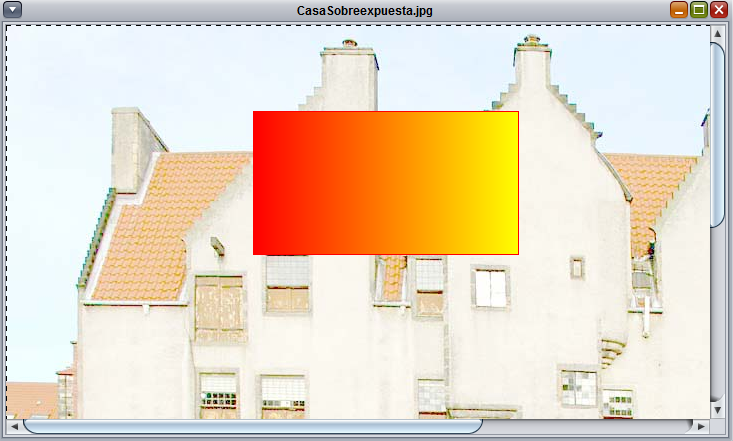
\includegraphics[scale=0.40]{images/ventanainterna}
  \caption{Ventana Interna}
  \label{Ventana Interna}
\end{figure}

\subsection{VentanaInternaGrabador}
Esta clase ( tambien hereda de javax.swing.JInternalFrame ) representa a la ventana que usa Java Sound API para grabar audio.Lo mas destacable de ella es el manejador de eventos que se usa para cambiar iconos.
\begin{figure}[H]
  \centering
    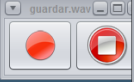
\includegraphics[scale=0.60]{images/ventanainternagrabador}
  \caption{Ventana Interna Grabador}
  \label{Ventana Interna Grabador}
\end{figure}

\begin{figure}[H]
  \centering
    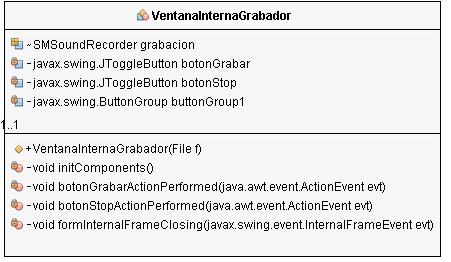
\includegraphics[scale=0.60]{images/ventanaInternaGrabador}
  \caption{UML VentanaInternaGrabador}
  \label{VentanaInternaGrabador}
\end{figure}

\begin{lstlisting}
class ManejadorAudio implements LineListener {
@Override

public void update(LineEvent event) {
    if (event.getType() == LineEvent.Type.START) {
      
    }
    if (event.getType() == LineEvent.Type.STOP) {
       
     
        VentanaInternaGrabador.this.botonStop.setSelected(true);
     }
    if (event.getType() == LineEvent.Type.CLOSE) {
       if(grabacion!=null) 
       grabacion.stop();
    }
    if(event.getType() == LineEvent.Type.OPEN){
        
    }
}
\end{lstlisting}
\subsection{VentanaInternaReproductor}
Esta clase representa a la ventana que usa Java Sound API para reproducir audio.El código es casi similar al anterior.
\begin{figure}[H]
  \centering
    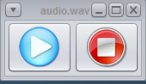
\includegraphics[scale=0.60]{images/ventanainternareproductor}
  \caption{Ventana Interna Reproductor}
  \label{Ventana Interna Reproductor}
\end{figure}

\begin{figure}[H]
  \centering
    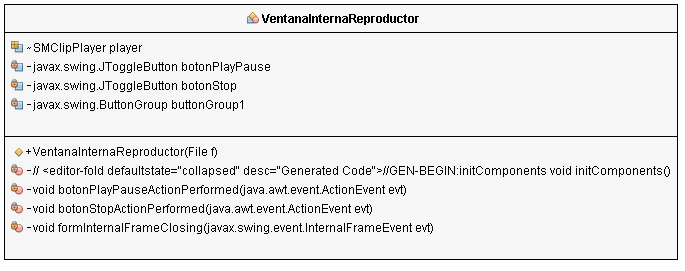
\includegraphics[scale=0.60]{images/ventanaInternaReproductor}
  \caption{UML VentanaInternaReproductor}
  \label{VentanaInternaReproductor}
\end{figure}


\subsection{VentanaInternaReproductorHebra}
Esta clase representa a la ventana que usa Java Sound API para reproducir audio, se añade un elemento \emph{JProgressBar}.Se destaca la creación de la clase \emph{VentanaInternaReproductorHebra} que implementa la interfaz \emph{Runnable} ( posteriormente se explica porque se opta por este diseño).

\begin{figure}[H]
  \centering
    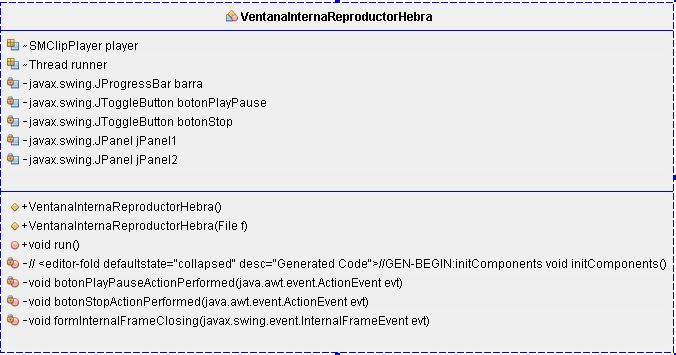
\includegraphics[scale=0.50]{images/ventanaInternaReproductorUML}
  \caption{UML VentanaInternaReproductorHebra}
  \label{VentanaInternaReproductor}
\end{figure}


\begin{lstlisting}

public class VentanaInternaReproductorHebra extends 
             javax.swing.JInternalFrame implements Runnable{

    /**
     * Creates new form VentanaInternaReproductorHebra
     */
   
    
 public VentanaInternaReproductorHebra() {
  initComponents();
  }
    
  SMClipPlayer player;
  Thread runner= null;

  /**
   * Constructor
   * @param f File
  */
  public VentanaInternaReproductorHebra(File f) {
     initComponents();
     player = new SMClipPlayer(f);
     player.setLineListener(new 
          VentanaInternaReproductorHebra.ManejadorAudio());
        
    }
 
 /**
  * Metodo run de la hebra que es invocado cuando se llama al metodo start 
  *del objeto hebra declarado
 */
 @Override
 public void run() {
   for(int x=0;x<100;x++){
      barra.setValue(x);
      barra.repaint();
            
      try{
        Thread.sleep(100);
      }catch(Exception e){
    }
  }
 }
        

/**
 * Recoge evento e inicia reproduccion
 * @param evt ActionEvent
 */
private void botonPlayPauseActionPerformed(java.awt.event.ActionEvent evt) {
  if(player!=null){
     player.play();

    if(runner==null){
      runner = new Thread(this);
      runner.start();
              
    }else{
      runner.resume();
 
     }
            
   }
        
}
/**
  * Recoge evento y para o corta reproduccion
  * @param evt ActionEvent
*/
 private void botonStopActionPerformed(java.awt.event.ActionEvent evt) {
   if(player!=null) player.stop();
    
     if(runner.isAlive()){
            
       runner.suspend();
       runner=null;
       barra.setValue(0);                   
    }
  
  }

\end{lstlisting}

%\begin{figure}[H]
%  \centering
%    \includegraphics[scale=0.60]{images/ventanainternareproductorhebra}
%  \caption{Ventana Interna Reproductor Hebra}
%  \label{Ventana Interna Reproductor Hebra}
%\end{figure}

\begin{figure}[H]
  \centering
    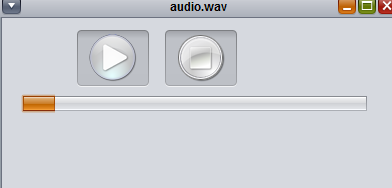
\includegraphics[scale=0.60]{images/VentanaInternaReproductorHebra}
  \caption{UML VentanaInternaReproductorHebra}
  \label{VentanaInternaReproductorHebra}
\end{figure}
\textbf{Figura}
\textbf{Nota: Por corregir, hay que adaptar avance barra al tiempo de duración del audio}.

\subsection{VentanaInternaJMFPlayer}
Con esta clase( tambien hereda de javax.swing.JInternalFrame ) se usa la API JMF para reproducción de audio y video.El constructor es privado, y por tanto se instancia para evitar excepciones que pudieran darse en el constructor.Se incluye el método getFrame para realizar capturas.
\begin{figure}[H]
  \centering
    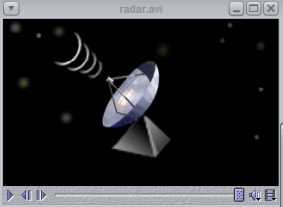
\includegraphics[scale=0.60]{images/ventanainternajmfp}
  \caption{Ventana Interna JMFPlayer}
  \label{Ventana Interna JMFPlayer}
\end{figure}

\begin{figure}[H]
  \centering
    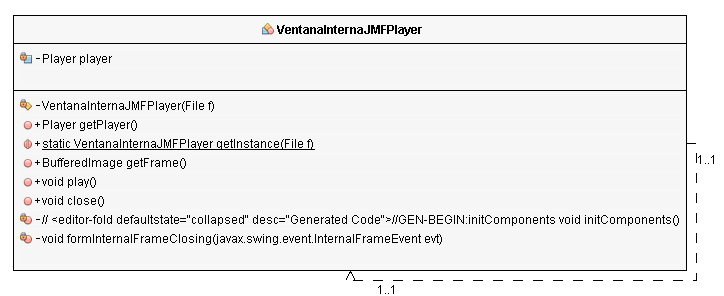
\includegraphics[scale=0.60]{images/ventanaInternaJMFPlayer}
  \caption{UML VentanaInternaJMFPlayer}
  \label{VentanaInternaJMFPlayer}
\end{figure}

\begin{lstlisting}
public BufferedImage getFrame(){
    FrameGrabbingControl fgc;
    String claseCtr = "javax.media.control.FrameGrabbingControl";
    fgc = (FrameGrabbingControl)player.getControl(claseCtr );
    Buffer bufferFrame = fgc.grabFrame();
    BufferToImage bti;
    bti=new BufferToImage((VideoFormat)bufferFrame.getFormat());
    Image img = bti.createImage(bufferFrame);
    return (BufferedImage)img;
   
}
\end{lstlisting}

\subsection{VentanaInternaCamara}
Al igual que antes se usa la API JMF pero en este caso para reproducir lo que capta la webcam.Por motivos que desconozco mi sistema no la reconoce, pero se ha probado en el ordenador del profesor y funciona.

\begin{figure}[H]
  \centering
    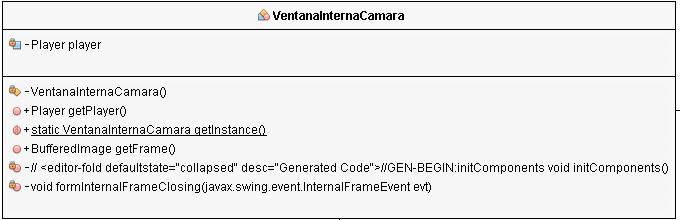
\includegraphics[scale=0.60]{images/ventanaInternaCamara}
  \caption{UML VentanaInternaCamara}
  \label{VentanaInternaCamara}
\end{figure}

\begin{lstlisting}
private VentanaInternaCamara() {
        initComponents();
         CaptureDeviceInfo deviceInfo;
        
       
        String dName="vfw:Microsoft WDM Image Capture (Win32):0";
        deviceInfo = CaptureDeviceManager.getDevice(dName);
       
        MediaLocator ml = deviceInfo.getLocator();
        
        
        try {
            player = Manager.createRealizedPlayer(ml);
            Component vc = player.getVisualComponent();
          
            if(vc!=null)add(vc, java.awt.BorderLayout.CENTER);
               player.start();
              
            }catch(Exception e) {
                System.err.println("VentanaInternaJMFPlayer: "+e);
                player = null;
}
    }
\end{lstlisting}
%---------------------------


%----------------
\section{Clases implementadas para las formas geometricas.(sm.fgm.graficos)}
Tanto la practica 3 como la 7 presentaban el problema de que todas las formas geométricas tenian los mismos atributos y por tanto limitaban el dibujado\cite{graphics} de ellas en el lienzo.Esto se ha solucionado creando clases propias de manera que en mi caso he creado una clase padre abstracta \textbf{Figura} que hereda de \emph{Shape} y que contiene los atributos de las diferentes formas geometricas, ademas contiene el metodo pintar dandole una vuelta de tuerca a lo que ocurría en las practicas 3 y 7, ahora si esta orientado a objetos que en este caso es la forma geometrica y por tanto este es uno de sus metodos.
Las clases hijas y por tanto que heredan de \textbf{Figura} son las diferentes formas geometricas que pueden darse, en mi caso he implementado las clases \textbf{MiLinea, MiRectangulo, MiCurva, MiRectanguloRedondeado, MiElipse}, estas implementan los metodos de Shape ( no se implementan en Figura ) y algunos propios que son necesario para su uso.
Una alternativa a esta propuesta es la de crear \emph{Figura} como una interfaz con los métodos comunes que despues tendran cada clase de figura geométrica,es decir, cada clase que hereda tendrá que implementar estos métodos pero ademas hay que declarar los atributos, cosa que no se puede realizar en la interfaz.

Por tanto las ventajas que encuentro al realizar la clase abstracta y heredar de ellas son:
\begin{itemize}
\item - No necesito implementar en cada clase metodos iguales ( repetir codigo ), con implementarlos en la clase abstracta es suficiente.Vease el método \emph{pintar} que es común a todas las figuras.
\item  Puedo definir los atributos que son similares en las clases de figuras en la clase abstracta.
\end{itemize}
Entre las desventajas encuentro:
\begin{itemize}
\item - Con la interfaz hubiese podido hacer uso de herencia multiple, es decir, la clase de la Figura hubiese podido implementar la interfaz y heredar de la clase Rectangle2D por ejemplo.
\end{itemize}

Por tanto y tras meditarlo mucho he considerado que la opcion de usar clase abstracta era la idonea ( no significa que la otra opcion sea mala), sobre todo porque a la hora de definir los atributos de las figuras y pintar era mucho mas comodo y me ahorraba hacer muchos \emph{instanceof}. 
\begin{figure}[H]
  \centering
    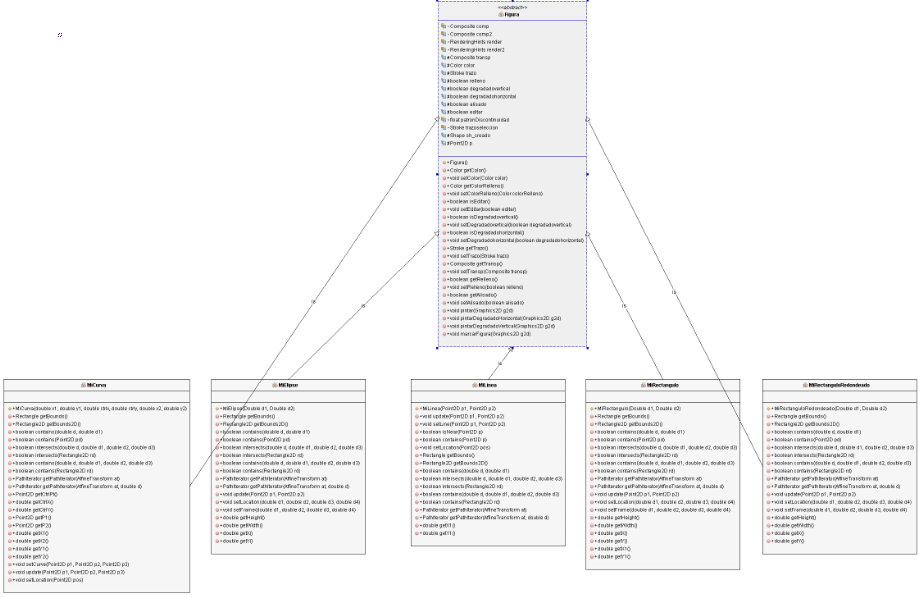
\includegraphics[scale=0.51]{images/smfgmgraficos2}
  \caption{Clases Geometricas sm.fgm.graficos}
  \label{Clases Geometricas sm.fgm.graficos}
\end{figure}

\subsection{Figura}
Como se comenta en el parrafo anterior, esta es una clase abstracta que hereda de Shape\cite{Shape} y que define los atributos de cada forma geométrica, es decir los atributos utilizados para el color, relleno, trazo,..., se declaran y por tanto despues son heredados . Su metodo principal es pintar y es usado por cada forma geométrica para pintarse.El modo editar se usa de la siguiente manera en la interfaz gráfica:
 Al seleccionar esta opción posteriormente se selecciona los atributos deseados y por último la figura a la que se le aplicará, pudiendose mover a otra posición del lienzo tambien.
\begin{lstlisting}

public  abstract class  Figura implements Shape{
   
    Composite comp=AlphaComposite.getInstance(AlphaComposite.SRC_OVER,0.5f);
    Composite comp2=AlphaComposite.getInstance(AlphaComposite.SRC);
    RenderingHints render= new RenderingHints(
    RenderingHints.KEY_ANTIALIASING,RenderingHints.VALUE_ANTIALIAS_ON);
    RenderingHints render2= new RenderingHints(
    RenderingHints.KEY_ANTIALIASING,RenderingHints.VALUE_ANTIALIAS_OFF);
    protected Composite transp;
    protected Color color,colorRelleno ;
    protected Stroke trazo ;
    protected boolean relleno;
    protected boolean degradadovertical;
    protected boolean degradadohorizontal;
    protected boolean alisado ;

    protected boolean editar;
    float patronDiscontinuidad[] = {15.0f, 15.0f};
    Stroke trazoseleccion = new BasicStroke(
    1.0f,BasicStroke.CAP_ROUND,BasicStroke.JOIN_MITER, 1.0f,
    patronDiscontinuidad, 0.0f);
    ...
    


 public void pintar(Graphics2D g2d){
        
        
        if(editar){
            marcarFigura(g2d);            
        }

            g2d.setStroke(this.getTrazo());
              g2d.setComposite(transp);

            if(this.getAlisado()){
              g2d.setRenderingHints(render);
              }
           
            if(this.getRelleno()){
                 g2d.setPaint(this.getColorRelleno());
                 
                 if(degradadohorizontal){
                     pintarDegradadoHorizontal(g2d); 
                     
                 }
                 if(degradadovertical){
                     pintarDegradadoVertical(g2d);                    
                 }
                 
                 g2d.fill(this);
            }
                g2d.setPaint(this.getColor());
                g2d.draw(this);
            g2d.setRenderingHints(render2); 
            g2d.setComposite(comp2);
        
    }
\end{lstlisting}
\begin{figure}[H]
  \centering
    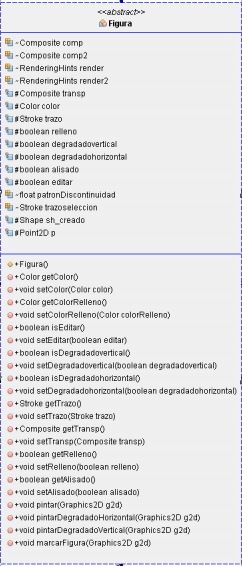
\includegraphics[scale=0.75]{images/figura2}
  \caption{Clase Figura}
  \label{Clases Figura}
\end{figure}
\subsection{MiLinea}
Esta clase\cite{Linea} hereda de \textbf{Figura} y por tanto sus atributos y metodos implementados. En ella se ha implementado los metodos de Shape que no habian sido implementados en la clase \textbf{Figura}.Me apoyo en la clase \emph{Line2D} para su implementación.
\begin{lstlisting}
   public MiLinea(Point2D p1, Point2D p2){
        super();
        sh_creado= new Line2D.Float(p1,p2);
    }
    
     public boolean isNear(Point2D p){
       if((((Line2D)sh_creado).getX1()!=((Line2D)sh_creado).getX2())||
            (((Line2D)sh_creado).getY1()!=((Line2D)sh_creado).getY2())){
        return ((Line2D)sh_creado).ptLineDist(p) <=2.0; 
        }
           
      return (Math.abs(((Line2D)sh_creado).getX1() - p.getX()))<=3.0;
      
        }
 
      @Override
    public boolean contains(Point2D p) {
        return isNear(p);
    }
    
     public void setLocation(Point2D pos){
      double dx=pos.getX()-((Line2D)sh_creado).getX1();
      double dy=pos.getY()-((Line2D)sh_creado).getY1();
      Point2D newp2 = new Point2D.Double(((Line2D)sh_creado).getX2()+dx,
      ((Line2D)sh_creado).getY2()+dy);
      
      ((Line2D)sh_creado).setLine(pos,newp2);
}
\end{lstlisting}
\begin{figure}[H]
  \centering
    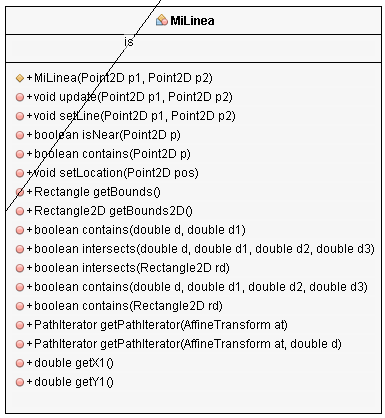
\includegraphics[scale=0.55]{images/milinea2}
  \caption{Clase MiLinea}
  \label{Clases MiLinea}
\end{figure}
Destacar los metodos \textbf{public boolean isNear(Point2D p)} y \textbf{public void setLocation(Point2D pos)}
\subsection{MiRectangulo}
Al igual que en el caso anterior hereda de \textbf{Figura}.Me apoyo en la clase \emph{Rectangle2D}\cite{Rectangulo} para su implementación.Los métodos heredados los he implementado de la siguiente forma ( en el resto de clases de forma similar a esta ):
\begin{lstlisting}

   public MiRectangulo(Double d1, Double d2){
        super();
        sh_creado= new Rectangle2D.Double(d1, d2, 0, 0);
        
    }
    
 @Override
    public Rectangle getBounds() {
       return ((Rectangle2D)sh_creado).getBounds();
    }

    @Override
    public Rectangle2D getBounds2D() {
        return ((Rectangle2D)sh_creado).getBounds2D();
    }

    @Override
    public boolean contains(double d, double d1) {
        return ((Rectangle2D)sh_creado).contains(d, d1); 
    }

    @Override
    public boolean contains(Point2D pd) {
        return ((Rectangle2D)sh_creado).contains(pd);
    }

    @Override
    public boolean intersects(double d, double d1, double d2, double d3) {
        return ((Rectangle2D)sh_creado).intersects(d, d1, d2, d3);
    }

    @Override
    public boolean intersects(Rectangle2D rd) {
        return ((Rectangle2D)sh_creado).intersects(rd); 
    }

    @Override
    public boolean contains(double d, double d1, double d2, double d3) {
        return ((Rectangle2D)sh_creado).contains(d, d1, d2, d3);
    }

    @Override
    public boolean contains(Rectangle2D rd) {
        return ((Rectangle2D)sh_creado).contains(rd);
    }

    @Override
    public PathIterator getPathIterator(AffineTransform at) {
        return ((Rectangle2D)sh_creado).getPathIterator(at);
    }

    @Override
    public PathIterator getPathIterator(AffineTransform at, double d) {
        return ((Rectangle2D)sh_creado).getPathIterator(at, d);
    }
         
    
\end{lstlisting}
\begin{figure}[H]
  \centering
    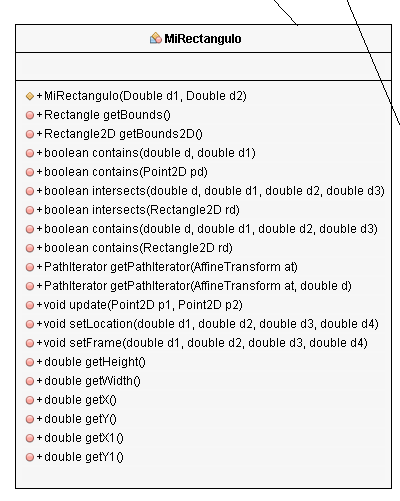
\includegraphics[scale=0.55]{images/mirectangulo2}
  \caption{Clase MiRectangulo}
  \label{Clases MiRectangulo}
\end{figure}
\subsection{MiRectanguloRedondeado}
Al igual que en el caso anterior hereda de \textbf{Figura}.En cierto modo similar a las clases \textbf{MiRectangulo} y \textbf{MiElipse}.Nuevamente me apoyo en otra clase para su implementacion\cite{Rectangulored}.
\begin{lstlisting}
  public MiRectanguloRedondeado(Double d1, Double d2){
        super();
        sh_creado= new RoundRectangle2D.Double(d1,d2,0,0,10,10);
 }
 
 public void update(Point2D p1, Point2D p2) {
        ((RoundRectangle2D)sh_creado).setFrameFromDiagonal(p1, p2);
  
    }

    public void setLocation(double d1,double d2,double d3,double d4){
        ((RoundRectangle2D)sh_creado).setFrame(d1, d2, d3, d4);
    }
    public void setFrame(double d1,double d2,double d3,double d4){
        ((RoundRectangle2D)sh_creado).setFrame(d1, d2, d3, d4);
    }
    public double getHeight(){
        return ((RoundRectangle2D)sh_creado).getHeight();
    }
    public double getWidth(){
        return ((RoundRectangle2D)sh_creado).getWidth();
    }
 
   public double getX(){ 
   return ((RoundRectangle2D)sh_creado).getX();
   }

   public double getY(){ 
    return ((RoundRectangle2D)sh_creado).getY();
   }
\end{lstlisting}
\begin{figure}[H]
  \centering
    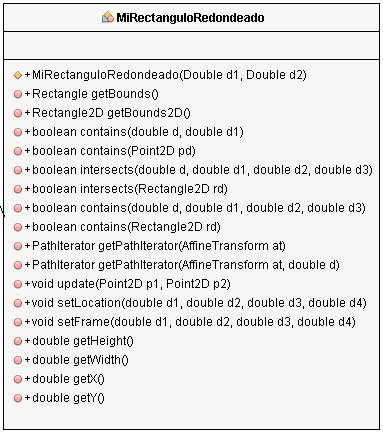
\includegraphics[scale=0.55]{images/mirectanguloredondeado2}
  \caption{Clase MiRectanguloRedondeado}
  \label{Clases MiRectanguloRedondeado}
\end{figure}
\subsection{MiElipse}
Al igual que en el caso anterior hereda de \textbf{Figura}.Al igual que en las anteriores, me apoyo en \emph{Ellipse2D} para su desarrollo\cite{Ellipse}
\begin{lstlisting}
  public MiElipse(Double d1, Double d2){
        super();
        sh_creado= new Ellipse2D.Double(d1,d2,0,0);
    }
    
         public void update(Point2D p1, Point2D p2) {
        
        ((Ellipse2D)sh_creado).setFrameFromDiagonal(p1, p2);
       
    }

      public void setLocation(double d1,double d2,double d3,double d4){
        ((Ellipse2D)sh_creado).setFrame(d1, d2, d3, d4);
    }
     
     public void setFrame(double d1,double d2,double d3,double d4){
        ((Ellipse2D)sh_creado).setFrame(d1, d2, d3, d4);
    }

    public double getHeight(){
        return ((Ellipse2D)sh_creado).getHeight();
    }
 
    public double getWidth(){
        return ((Ellipse2D)sh_creado).getWidth();
    } 
 
   public double getX(){ 
    return ((Ellipse2D)sh_creado).getX();
   }
  
   public double getY(){ 
    return ((Ellipse2D)sh_creado).getY();
   }
\end{lstlisting}
\begin{figure}[H]
  \centering
    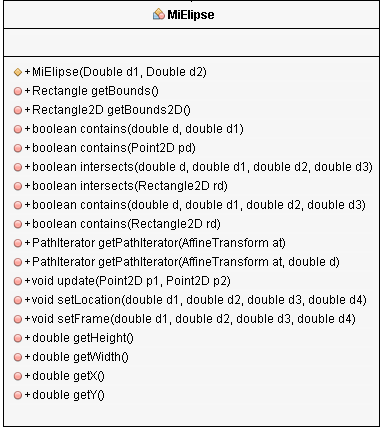
\includegraphics[scale=0.55]{images/mielipse2}
  \caption{Clase MiElipse}
  \label{Clases MiElipse}
\end{figure}
\subsection{MiCurva}
Al igual que en el caso anterior hereda de \textbf{Figura}.A tener en cuenta para su manejo el punto de control\cite{Curva} que será donde se realice la 'curva' y que implica que se dibuje en dos pasos, es decir, primero se dibuja una recta y despues se establece el punto de control como puede observarse en los eventos \emph{pressed, dragged y released } del \emph{lienzo}.
\begin{lstlisting}
 public void setCurve(Point2D p1,Point2D p2,Point2D p3){
        //((QuadCurve2D)sh_creado).setCurve(x1, y1, ctrlx, ctrly, x2, y2);
        ((QuadCurve2D)sh_creado).setCurve(p1, p2, p3);
    }
    
   public void setCurve(Point2D p1,Point2D p2,Point2D p3){
        //((QuadCurve2D)sh_creado).setCurve(x1, y1, ctrlx, ctrly, x2, y2);
        ((QuadCurve2D)sh_creado).setCurve(p1, p2, p3);
    }
 
    public void update(Point2D p1,Point2D p2,Point2D p3){
        //((QuadCurve2D)sh_creado).setCurve(x1, y1, ctrlx, ctrly, x2, y2);
        ((QuadCurve2D)sh_creado).setCurve(p1, p2, p3);
    }
    
 
    public void setLocation(Point2D pos){
        Point2D p_aux=null;
        Point2D p_aux_control=null;
        double dist_x,dist_y;
        
         dist_x = pos.getX() - ((QuadCurve2D)sh_creado).getX1();
         dist_y = pos.getY() - ((QuadCurve2D)sh_creado).getY1();
         p_aux = new Point2D.Double( ((QuadCurve2D)sh_creado).getX2()+dist_x, 
              ((QuadCurve2D)sh_creado).getY2()+dist_y);
         p_aux_control = new Point2D.Double(((QuadCurve2D)sh_creado).getCtrlX()
             +dist_x,((QuadCurve2D)sh_creado).getCtrlY()+dist_y);
      
         setCurve(pos,p_aux_control, p_aux);
                   
    }  
\end{lstlisting}
\begin{figure}[H]
  \centering
    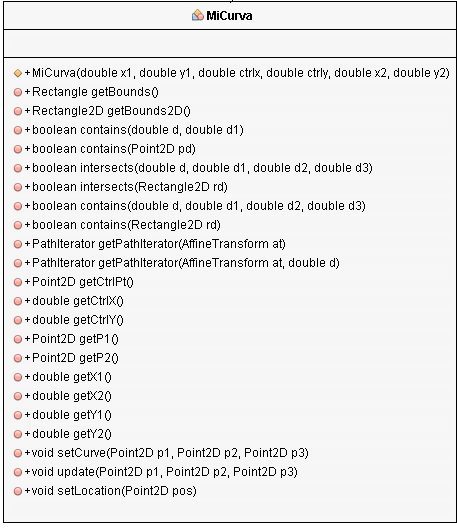
\includegraphics[scale=0.55]{images/micurva2}
  \caption{Clase MiCurva}
  \label{Clases MiCurva}
\end{figure}
%-----------------------------------------------------------

%------------------------------------------------------
%----------------------------------------------------------------------------------------
%	Cuesti´on 2
%----------------------------------------------------------------------------------------
\section{Clases utilizadas para el dibujado de formas geométricas e imágenes.(sm.fgm.iu)}
En esta sección se explica las dos clases utilizadas para el manejo( utilizacion de los metodos ) de las clases geometricas e imagenes ( realmente las imagenes se manejan desde la VentanaPrincipal utilizando el objeto lienzo y sus metodos).
\subsection{Lienzo2Dfinal} 
Esta clase es la que recoge y muestra las figura geométricas en pantalla a traves del metodo \emph{public void paint(Graphics g)} , esto se consigue recogiendo los eventos( seleccion de color, trazo,..) de \emph{VentanaPrincipal} y vinculandolos al objeto que se desea dibujar ( estos objetos tienen los atributos color, trazo, transparencia,...), a su vez se guarda en un array de figuras que será lo que se recorra en dicho metodo.
\begin{figure}[H]
  \centering
    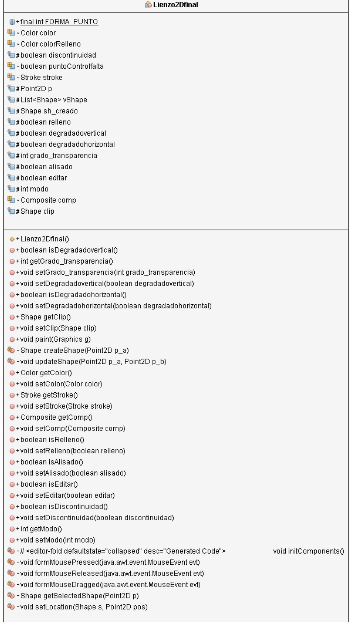
\includegraphics[scale=0.75]{images/lienzo2dfinal}
  \caption{UML Lienzo2Dfinal}
  \label{UML Lienzo2Dfinal}
\end{figure}
Destacar los tres eventos utilizados para la creación de la figura geometrica:
\begin{itemize}
\item \textbf{formMousePressed} - Corresponde a pulsar el botón izquierdo del ratón.
\item \textbf{formMouseDragged} - Corresponde a arrastrar con el botón pulsado.
\item \textbf{formMouseReleased} - Corresponde a soltar el botón del ratón.
\end{itemize}

\subsection*{public void paint(Graphics g)}
En este método se recorre el array de figuras geómetricas y se llama al metodo \emph{pintar} de cada uno de ellos pasandole un objeto \emph{Graphics2D} como argumento.
\begin{lstlisting}
public void paint(Graphics g){
        super.paint(g);
        Graphics2D g2d = (Graphics2D)g;
        
        if (this.clip != null) {
             g2d.clip(this.clip);
         }
        for(Shape s:vShape) {
            ((Figura)s).pintar(g2d);
                        
        }
}
\end{lstlisting}

\subsection*{private Shape createShape(Point2D p\_a)}
Crea el objeto seleccionado en \emph{VentanaPrincipal} con los atributos correspondientes.
\begin{lstlisting}
 private Shape createShape(Point2D p_a){
     
        if(p_a==null){
            return null;
        }
      
        if(modo==0){
             sh_creado= new MiLinea(p_a,p_a);
              //punto con las mismas coordenadas, asi crea punto en vez linea           
         }else if(modo==1){
             sh_creado= new MiLinea(p_a,p_a); // linea           
         }else if(modo==2){  
            sh_creado= new MiRectangulo(p_a.getX(),p_a.getY());
         }else if(modo==3){ 
             sh_creado= new MiElipse(p_a.getX(),p_a.getY());
         }else if(modo==4){  
            sh_creado= new MiRectanguloRedondeado(p_a.getX(),p_a.getY());   
         }else if(modo==5){  
            sh_creado= new MiCurva(p_a.getX(),p_a.getY(),p_a.getX(),p_a.getY(),p_a.getX(),p_a.getY());  
            p3=p_a;
         }else{      
             sh_creado=null;
         }
        
   if(sh_creado!=null){
      ((Figura)sh_creado).setColor(this.color);
      ((Figura)sh_creado).setTrazo(this.stroke);
      ((Figura)sh_creado).setAlisado(this.alisado);
      ((Figura)sh_creado).setRelleno(this.relleno);
      ((Figura)sh_creado).setColorRelleno(this.colorRelleno);
      ((Figura)sh_creado).setDegradadohorizontal(this.degradadohorizontal);
      ((Figura)sh_creado).setDegradadovertical(this.degradadovertical);
      ((Figura)sh_creado).setTransp(this.comp);
      ((Figura)sh_creado).setEditar(this.editar);
        }
        return sh_creado;
    }
\end{lstlisting}

\subsection*{private void updateShape(Point2D p\_a, Point2D p\_b)}
Usado para actualizar las formas geométricas al llamar al \emph{dragged}.
\begin{lstlisting}
private void updateShape(Point2D p_a, Point2D p_b){
    if (sh_creado instanceof MiLinea) {        
      ((MiLinea)sh_creado).update(p_a, p_b);
    }else if(sh_creado instanceof MiRectangulo) {
      ((MiRectangulo)sh_creado).update(p_a, p_b);
    }else if(sh_creado instanceof MiElipse) {
      ((MiElipse)sh_creado).update(p_a, p_b);
    }else if(sh_creado instanceof MiRectanguloRedondeado) {
      ((MiRectanguloRedondeado)sh_creado).update(p_a, p_b);  
    }else if(sh_creado instanceof MiCurva) {
      ((MiCurva)sh_creado).update(p_a,p_b, p2);    
    }else if(sh_creado instanceof RectangularShape) {
      ((RectangularShape)sh_creado).setFrameFromDiagonal(p_a, p_b);
    }
 
    }
\end{lstlisting}

\subsection*{private void formMousePressed(java.awt.event.MouseEvent evt)}
Corresponde al evento que se produce cuando se pulsa el boton izquierdo del raton, en este método se distingue si esta editando o no. En el modo que no edita se diferencia dos casos, un primer caso donde puede corresponder a la curva ya pintada donde solo queda establecer el punto de control o un segundo caso donde se crea la figura geometrica mediante la llamada a \emph{createShape} ( notar que se definen los atributos ).
El segundo caso corresponde al modo editar donde se calcula el sitio geográfico del punto p4 con el objetivo de evitar el 'efecto ancla' al editar.
\begin{lstlisting}
private void formMousePressed(java.awt.event.MouseEvent evt) {                                  
  p4=new Point2D.Double();
  p = evt.getPoint();
      
        
  if(editar){
    this.sh_creado =  getSelectedShape(p);
            
    if(sh_creado!=null){
       double x=0,y=0;
       if (sh_creado instanceof MiLinea){
         x=((MiLinea)sh_creado).getX1();
         y=((MiLinea)sh_creado).getY1();

       }else
         if (sh_creado instanceof MiRectangulo){
          x=((MiRectangulo)sh_creado).getX();
          y=((MiRectangulo)sh_creado).getY();

       }else if (sh_creado instanceof MiElipse){
          x=((MiElipse)sh_creado).getX();
          y=((MiElipse)sh_creado).getY();

       }else if (sh_creado instanceof MiRectanguloRedondeado){
          x=((MiRectanguloRedondeado)sh_creado).getX(); 
          y=((MiRectanguloRedondeado)sh_creado).getY();  

       }else if (sh_creado instanceof MiCurva){
          x= ((MiCurva)sh_creado).getX1();
          y= ((MiCurva)sh_creado).getY1();
       }
               
       p4.setLocation(x - p.getX(), y- p.getY()); 
      }
            
     if(sh_creado!=null){
       ((Figura)sh_creado).setColor(this.color);
       ((Figura)sh_creado).setTrazo(this.stroke);
       ((Figura)sh_creado).setAlisado(this.alisado);
       ((Figura)sh_creado).setRelleno(this.relleno);
       ((Figura)sh_creado).setColorRelleno(this.colorRelleno);
       ((Figura)sh_creado).setDegradadohorizontal(this.degradadohorizontal);
       ((Figura)sh_creado).setDegradadovertical(this.degradadovertical);
       ((Figura)sh_creado).setTransp(this.comp);
       ((Figura)sh_creado).setEditar(this.editar);
      }
} else{
   if((modo==FORMA_CURVA)&&(puntoControlfalta)){
     if((Figura)vShape.get(vShape.size()-1) instanceof MiCurva){
                
     ((MiCurva)vShape.get(vShape.size()-1)).update(p3, evt.getPoint(), p2);
       }
    }else{
        Shape nuevo_s= createShape(p);
        vShape.add(nuevo_s);
     }
  } 
}    
\end{lstlisting}
\subsection*{private void formMouseReleased(java.awt.event.MouseEvent evt)}
Corresponde al evento de soltar el boton izquierdo,en el nuevamente se distinguen dos casos.En el modo editar se establece el cursor por defecto y se pone con valor a false la booleana editar de la figura geometrica con el objetivo de quitar el boundingbox ( el recuadro desaparece cuando dejemos de editar ).En el modo de no editar o bien se termina de dibujar la curva o se termina las otras figuras salvo que sea la curva donde se usa una booleana para indicar que falta establecer el punto de control. 
\begin{lstlisting}
private void formMouseReleased(java.awt.event.MouseEvent evt) {                                   
        
  if (editar) {
     setCursor(Cursor.getDefaultCursor());
     if(sh_creado!=null){
       ((Figura)sh_creado).setEditar(false);
     }         
 }else{
    if((modo==FORMA_CURVA)&&(puntoControlfalta)){
      ((MiCurva)sh_creado).update(p3, evt.getPoint(), p2);
       puntoControlfalta=false;
       repaint();
    }else{  
       puntoControlfalta=true;
       this. formMouseDragged(evt);  
    }
  }
 }      
\end{lstlisting}
\subsection*{private void formMouseDragged(java.awt.event.MouseEvent evt}
Evento que corresponde a arrastrar el raton con el boton pulsado.Nuevamente se distinguen dos casos, el modo edicion y el modo donde no se edita.
En el modo edición se mueve la figura al lugar donde se desee mientras que en el modo de no edicion se distinguen tres casos:
\begin{itemize}
\item Un primer caso donde solo falta establecer el punto de control de la curva
\item Un segundo caso donde todavia no es necesario el punto de control sino acabar de definir el primer paso de construccion de la curva que es realizar la recta.
\item El tercer caso es el resto de las opciones, un caso generico para la linea, rectangulo, elipse,..., donde se actualiza la figura.
\end{itemize}
\begin{lstlisting}
 private void formMouseDragged(java.awt.event.MouseEvent evt) {                                  
     Point2D punto = evt.getPoint();
            
     if(editar){
                       
         if(sh_creado!=null){
                      
            setLocation(sh_creado,
              new Point2D.Double(evt.getX()+p4.getX(),evt.getY()+p4.getY())); 
         }
    } else if (modo != 0) {//el punto no se actualiza{
      if((modo==FORMA_CURVA)&&(puntoControlfalta)
         &&(sh_creado instanceof MiCurva)){
                       
         ((MiCurva)sh_creado).update(p3,punto, p2);
      }else if((modo==FORMA_CURVA)&&!(puntoControlfalta)){
           p2=evt.getPoint();
           updateShape(p, punto);
      }else{
          puntoControlfalta = false;
          updateShape(p, punto);
      }
  }
    
             
        repaint();
    }     
\end{lstlisting}

\subsection*{private Shape getSelectedShape(Point2D p)}
Este metodo es usado en el editar del Pressed para saber que figura se esta editando.
\begin{lstlisting}
 private Shape getSelectedShape(Point2D p){
    for(Shape s:vShape)
       if(s.contains(p)) return s;
          return null;
}
\end{lstlisting}

\subsection*{private void setLocation(Shape s, Point2D pos)}
Sirve para actualizar la figura cuando se realiza el dragged.
\begin{lstlisting}
private void setLocation(Shape s, Point2D pos){
  if (s instanceof MiLinea){
     ((MiLinea)s).setLocation(pos);
  }else if (s instanceof MiRectangulo){
           
    ((MiRectangulo)s).setLocation(pos.getX(), pos.getY(), 
       ((MiRectangulo)s).getWidth(), ((MiRectangulo)s).getHeight());
  }else if (s instanceof MiElipse){
           
   ((MiElipse)s).setLocation(pos.getX(), pos.getY(), 
      ((MiElipse)s).getWidth(),((MiElipse)s).getHeight());
  }else if (s instanceof MiRectanguloRedondeado)
     ((MiRectanguloRedondeado)s).setLocation(pos.getX(), pos.getY(), 
        ((MiRectanguloRedondeado)s).getWidth(),
        ((MiRectanguloRedondeado)s).getHeight()); 
  }else if (s instanceof MiCurva){
            
    ((MiCurva)s).setLocation(pos);
          
  }else if(s instanceof RectangularShape){
    ((RectangularShape)s).setFrame(pos.getX(), pos.getY(), 
       ((RectangularShape)s).getWidth(),((RectangularShape)s).getHeight());
       
        }
}
\end{lstlisting}

\subsection{Lienzo2DImagenfinal}
Clase que hereda de \emph{Lienzo2Dfinal} y es la que se usa en \emph{VentanaInterna}, por tanto hereda los metodos de estas permitiendo dibujar sobre el lienzo o bien sobre una imagen cargada ( Lienzo2Dfinal no permite cargar una imagen ).Sobre esta imagen se pueden efectuar operaciones de rotacion, umbralización, etc.

\begin{figure}[H]
  \centering
    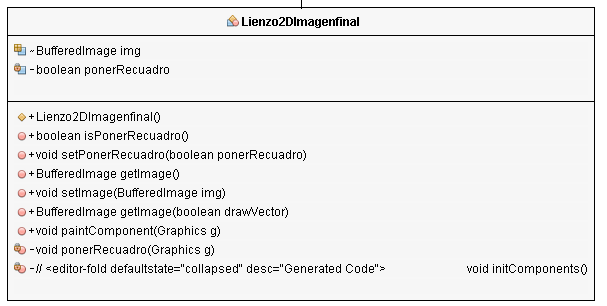
\includegraphics[scale=0.75]{images/lienzo2dimagenfinal}
  \caption{UML Lienzo2DImagenfinal}
  \label{UML Lienzo2DImagenfinal}
\end{figure}

\subsubsection*{public void setImage(BufferedImage img)}
Con este método se carga la imagen con su correspondiente clip ( rectangulo ).
\begin{lstlisting}
 public void setImage(BufferedImage img) {
    this.img = img;
    if(img!=null) {
        setPreferredSize(new Dimension(img.getWidth(),
          img.getHeight()));        
        Rectangle r = new Rectangle(0, 0, img.getWidth(), img.getHeight());
        setClip(r);
}
    }
\end{lstlisting}

\subsection*{public void paintComponent(Graphics g)}
La implementación por defecto del método paint de la clase JComponent llama, en este orden, a los métodos paintComponent, paintBorder y paintChildren. Este método contiene el código que determina cómo se pinta el componente, con ello se consigue dibujar encima de la imagen.
\begin{lstlisting}
public void paintComponent(Graphics g){
   super.paintComponent(g);//llama al paint de lienzo2Dfinal que es el padre
   if(img!=null)
     g.drawImage(img,0,0,this);
   if ((this.clip != null) && (this.ponerRecuadro)) {
                ponerRecuadro(g);
         }
    }
\end{lstlisting}

\section{Operaciones Propias}
En esta sección se explican las diferentes operaciones propias\cite{apuntestimd} ( desarrolladas en clases ) que se han utilizado para la parte de imágenes, algunas de ellas puede observarse que heredan de la clase abstracta \emph{BufferedImageOpAdapter} donde solo es necesario implementar el método \emph{filter}.

\subsection*{public class ConversionGrisOp extends BufferedImageOpAdapter}
En esta clase se realiza una conversión de la imagen pasandola de color a tonalidad de grises.Esto se consigue multiplicando cada banda RGB por los factores 0.299, 0.587 y 0.114 respectivamente.

\begin{figure}[H]
  \centering
    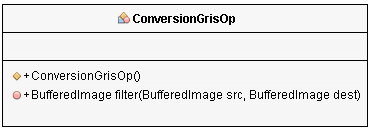
\includegraphics[scale=0.75]{images/conversiongris}
  \caption{UML ConversionGrisOp}
  \label{UML ConversionGrisOp}
\end{figure}

\begin{lstlisting}
 @Override
public BufferedImage filter(BufferedImage src, BufferedImage dest){
  if (src == null) {
    throw new NullPointerException("Imagen fuente a null");
   }
    
  if (dest == null) {
    dest = createCompatibleDestImage(src, null);
   }

  double[] color={255.0,255.0,255.0};
         
  WritableRaster srcRaster = src.getRaster();
  WritableRaster destRaster = dest.getRaster();
  
for (BufferedImagePixelIterator it = new BufferedImagePixelIterator(src); 
         it.hasNext();) {
    BufferedImagePixelIterator.PixelData pixel = it.next();
    //a las 3 bandas le asigno mismo valor
   color[0]=color[1]=color[2]=
          (int) ((0.299*pixel.sample[0])+(0.587*pixel.sample[1])+
                 (0.114*pixel.sample[2]));
   destRaster.setPixel(pixel.col, pixel.row, color);
   }
      return dest;
  }       
        }
\end{lstlisting}

\subsection*{public class EliminacionMitadBandaCentralOp extends BufferedImageOpAdapter}
En esta clase propia lo que se ha realizado es la reducción de la banda central a la mitad.Por tanto en las bandas RGB se reduce G a 0.5 de su valor.

\begin{figure}[H]
  \centering
    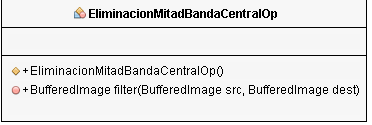
\includegraphics[scale=0.75]{images/eliminarbanda}
  \caption{UML EliminarMitadBandaCentralOp}
  \label{UML EliminarMitadBandaCentralOp}
\end{figure}

\begin{lstlisting}
  @Override
public BufferedImage filter(BufferedImage src, BufferedImage dest) {
  if (src == null) {
     throw new NullPointerException("Imagen fuente a null");
  }
    
  if (dest == null) {
     dest = createCompatibleDestImage(src, null);
   }

  double[] color={255.0,255.0,255.0};
         
  WritableRaster srcRaster = src.getRaster();
  WritableRaster destRaster = dest.getRaster();
        
  for (BufferedImagePixelIterator it = new BufferedImagePixelIterator(src); 
      it.hasNext();) {
    BufferedImagePixelIterator.PixelData pixel = it.next();
    color[0]=(int) (pixel.sample[0]);
    color[2]=(int) (pixel.sample[2]);
    color[1]=(int) (0.5*pixel.sample[1]);
    destRaster.setPixel(pixel.col, pixel.row, color);
            
 }
        
    return dest;
  } 
\end{lstlisting}

\subsection*{public class FiltroSeno}
Consiste en aplicar un filtro seno\cite{apuntessmm} a una imagen.

\begin{figure}[H]
  \centering
    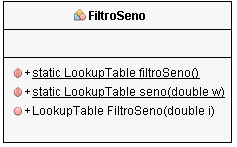
\includegraphics[scale=0.75]{images/filtroseno}
  \caption{UML FiltroSeno}
  \label{UML FiltroSeno}
\end{figure}

\begin{lstlisting}
 public static LookupTable seno(double w)
  {
double K = 255.0;
byte[] lt = new byte[256];
    
for (int i = 0; i <= 255; i++) {
  lt[i] = ((byte)(int)(K * Math.abs(Math.sin(Math.toRadians(i * w)))));
   }
 ByteLookupTable lookdevuelto = new ByteLookupTable(0, lt);
    
return lookdevuelto;
    
  }
 \end{lstlisting} 
 
\subsection*{public class PotenciaNesima}
 Consiste en aplicar un filtro potencia a una imagen segun un valor N introducido.
 
\begin{figure}[H]
  \centering
    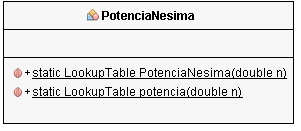
\includegraphics[scale=0.75]{images/potencia}
  \caption{UML PotenciaNesima}
  \label{UML PotenciaNesima}
\end{figure}

 \begin{lstlisting}
 public static LookupTable potencia(double n)
  {
  double K = 255.0/(Math.pow(255,n));
  byte[] lt = new byte[256];
    
  for (int i = 0; i <= 255; i++) {
    lt[i] = ((byte)(int)(K*Math.pow(i,n)));
  }
 ByteLookupTable lookdevuelto = new ByteLookupTable(0, lt);
    
 return lookdevuelto;
    
}
\end{lstlisting}

\subsection*{public class RaizNesima}
Se aplica filtro Raiz a una imagen segun un valor N introducido.

\begin{figure}[H]
  \centering
    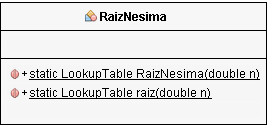
\includegraphics[scale=0.75]{images/raiz}
  \caption{UML RaizNesima}
  \label{UML RaizNesima}
\end{figure}


\begin{lstlisting}
 public static LookupTable raiz(double n)
  {
 double K = 255.0/(Math.pow(255,n));
 byte[] lt = new byte[256];
    
 for (int i = 0; i <= 255; i++) {
   lt[i] = ((byte)(int)(Math.pow((i/K),(1/n))));
  }
 ByteLookupTable lookdevuelto = new ByteLookupTable(0, lt);
    
  return lookdevuelto;
    
  }
\end{lstlisting}

\subsection*{public class RestaOp extends BinaryOp}
Operación binaria para visualizar diferencias entre dos imágenes.Lo realmente interesante es la implementacion del método heredado \emph{binaryOp} ( método abstracto de la clase BinaryOp).

\begin{figure}[H]
  \centering
    
\includegraphics[scale=0.75]{images/resta}
  \caption{UML RestaOp}
  \label{UML RestaOp}
\end{figure}

\begin{lstlisting}
 public int binaryOp(int v1, int v2){
    int rdo = v1-v2;
    if(rdo<=0) rdo=0;
    else if(rdo>=255) rdo=255;
    return rdo;
}
\end{lstlisting}

\subsection*{public class SumaOp extends BinaryOp}
Operación de blending que permite mezclar imágenes.

\begin{figure}[H]
  \centering
    
\includegraphics[scale=0.75]{images/suma}
  \caption{UML SumaOp}
  \label{UML SumaOp}
\end{figure}

\begin{lstlisting}
 public int binaryOp(int v1, int v2){
    int rdo = (int)((alpha*v1)+((1-alpha)*v2));
    if(rdo<=0) rdo=0;
    else if(rdo>=255) rdo=255;
    return rdo;
}
\end{lstlisting}

\subsection*{public class TintadoOp extends BufferedImageOpAdapter}
Clase que hereda de \emph{BufferedImageOpAdapter} y que entre otros implementa el método abstracto filter.En esta operación se efectua una transformacion en cada pixel tintandolo de un color determinado.

\begin{figure}[H]
  \centering
    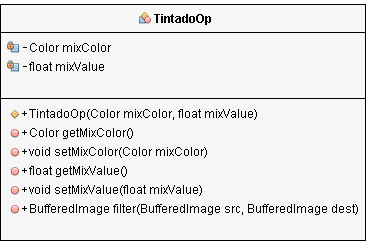
\includegraphics[scale=0.75]{images/tintado}
  \caption{UML TintadoOp}
  \label{UML TintadoOp}
\end{figure}

\begin{lstlisting}
 public BufferedImage filter(BufferedImage src, BufferedImage dest){
   if (dest == null) {
     dest = createCompatibleDestImage(src, null);
   }
   if (src == null) {
     throw new NullPointerException("Imagen fuente a null");
   }
  WritableRaster destRaster = dest.getRaster();
  float mixColorComp[] = mixColor.getColorComponents(null);

 for (BufferedImageSampleIterator it = 
      new BufferedImageSampleIterator(src); it.hasNext();) {
           
    BufferedImageSampleIterator.SampleData sample = it.next();
    float colorBand= 255 * mixColorComp[sample.band];
    sample.value = ((int) (sample.value * (1.0f - mixValue) + colorBand * mixValue));
    destRaster.setSample(sample.col, sample.row, sample.band, sample.value);
            
  }

  return dest;
    }
\end{lstlisting}  

\subsection*{public class TransformacionLogaritmica}
Se aplica un filtro logaritmico a la imagen.

\begin{figure}[H]
  \centering
    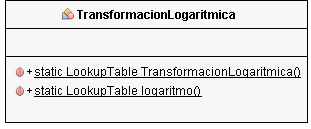
\includegraphics[scale=0.75]{images/logaritmica}
  \caption{UML TransformacionLogaritmica}
  \label{UML TransformacionLogaritmica}
\end{figure}

\begin{lstlisting}
 public static LookupTable logaritmo()
  {
  double c = (255.0/Math.log(256));
  byte[] lt = new byte[256];
    
  for (int i = 0; i <= 255; i++) {
    lt[i] = ((byte)(int)(c * Math.log(i+1)));
  }
  ByteLookupTable lookdevuelto = new ByteLookupTable(0, lt);
    
  return lookdevuelto;
    
  }
\end{lstlisting}  

\subsection*{public class UmbralizacionOp extends BufferedImageOpAdapter}
Clase que hereda de \emph{BufferedImageOpAdapter} y realiza una umbralización en escala de grises( para color se ha usado la aportada en la asignatura ).

\begin{figure}[H]
  \centering
    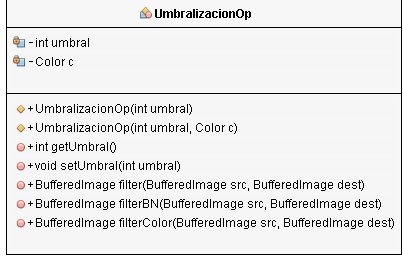
\includegraphics[scale=0.75]{images/umbralizacion}
  \caption{UML UmbralizacionOp}
  \label{UML UmbralizacionOp}
\end{figure}

\begin{lstlisting}
/*metodo usado en filter*/
public BufferedImage filterBN(BufferedImage src, BufferedImage dest){
     
  WritableRaster srcRaster = src.getRaster();
  WritableRaster destRaster = dest.getRaster();
        
 for (BufferedImagePixelIterator it = 
    new BufferedImagePixelIterator(src); it.hasNext();) {
    BufferedImagePixelIterator.PixelData pixel = it.next();
           
   int[] blanco=new int[pixel.numSamples];
   Arrays.fill(blanco,255);
            
   int[] negro=new int[pixel.numSamples]; //creo array con esa dimension
   Arrays.fill(negro,0);//rellena el array de valor 0
            
   int suma=0;
   for (int i = 0;i<pixel.numSamples;i++){
      suma+= pixel.sample[i];
   }
     suma/=pixel.numSamples;
            
    if(suma>=umbral){
      destRaster.setPixel(pixel.col, pixel.row, blanco);
               
    }else{
       destRaster.setPixel(pixel.col, pixel.row, negro);
    }   
}
        
    return dest;
}
\end{lstlisting}


\section{Uso de Hebras}
En esta sección se explica el uso de hebras para el reproductor de audio, haciendose hincapie en explicar el porqué se ha usado de una manera determinada. 
La finalidad de usar \emph{hebras} es permitir ejecutar de manera independiente un conjunto de instrucciones desde principio a fin, es lo que se llama \emph{programación paralela}.Un caso muy recomendado es cuando es necesario la realización de animaciones( en este caso el avance continuo de una barra de progreso).

Una hebra no es mas que un objeto \textbf{Thread} y hay dos maneras de crearlas \cite{ApuntesSCD}:

\begin{itemize}
\item Definiendo una subclase de \emph{Thread} \cite{hebras} ( heredando de esta ) y sobrecargando el método \emph{run()}
\item Definiendo una clase que implemente la interfaz \emph{Runnable} donde se declara una instancia de \emph{Thread} por cada hebra a ejecutar. Esto permitirá mayor flexibilidad.
\end{itemize}

Por esta segunda opción es la que me he decantado debido a que permite el uso de herencia multiple, en el caso de \emph{VentanaPrincipal} se podia haber hecho tal que así \emph{public class VentanaPrincipal extends javax.swing.JFrame implements Runnable} pero hay que tener en cuenta que solo habría un metodo \emph{run()} en ella y que todas las hebras que se usen tendrían que invocarse con ese único método( limitaría el uso de hebras en la aplicación ), por ello he decidido crear una clase que implementa \emph{Runnable} dentro de la clase \emph{VentanaPrincipal}  ( en \emph{VentanaInternaReproductorHebra} se ha optado por heredar de \emph{JInternalFrame} e implementar la interfaz \emph{Runnable}, esto hace que las hebras que se declaren solo puedan invocarse con un único metodo \emph{run()}). En definitiva se ha optado por permitir herencia multiple y poder incorporar otras hebras en la aplicación en un futuro si fuese necesario en \emph{VentanaPrincipal}.
A destacar en el caso de que se usen diferentes hebras la recomendación de sincronizarlas mediante el uso de cerrojos con el cualificador \emph{synchronized} o con una solución de alto nivel como son los \emph{monitores de Hoare}

\subsection{Reproductor de la VentanaPrincipal}
He implementado los botones de \emph{Open},\emph{Play},\emph{Pause} y \emph{Stop} en la \emph{VentanaPrincipal}, donde :
\begin{itemize}
\item El boton de \emph{Play} es el encargado de reproducir audio e inicializar el avance de la barra de progreso ( inicializa el objeto de la clase \emph{Hilo} sino lo estuviese).
\item El boton de \emph{Pause} es el encargado de pausar la reproduccion de audio y el avance de la barra de progreso.
\item El boton de \emph{Stop} es el encargado de parar la reproduccion de audio y vuelve la barra de progreso a su estado inicial( establece el objeto de la clase \emph{Hilo} a null).
\end{itemize}

\begin{figure}[H]
  \centering
    
\includegraphics[scale=0.75]{images/barraprogreso2}
  \caption{Barra de Progreso}
  \label{Barra de Progreso}
\end{figure}

\begin{lstlisting}
public class VentanaPrincipal extends javax.swing.JFrame {
   private BufferedImage imgFuente;
   SMClipPlayer player;
   Hilo hebra=null;
   
   ....

 private void openActionPerformed(java.awt.event.ActionEvent evt) {
   JFileChooser dlg = new JFileChooser();  
   String extension[]={"wav","au","aif"};  
   FileNameExtensionFilter filtro = new 
                FileNameExtensionFilter("Audio[wav,au,aif]",extension);
   dlg.setFileFilter(filtro);
    
    
   int resp = dlg.showOpenDialog(this);
   if (resp == JFileChooser.APPROVE_OPTION) {
      
     try
     {
      File f = dlg.getSelectedFile();
      player = new SMClipPlayer(f);
      if((hebra!=null)||(barraProgreso.getValue()!=0)){
        hebra.thr.suspend();
        barraProgreso.setValue(0);
        hebra=null;
      }
     }
     catch (Exception ex)
     {
     System.err.println("Error");
     }
   }  
    }

private void playActionPerformed(java.awt.event.ActionEvent evt) {
   if(player!=null){
     player.play();
        
     if(hebra==null){
       hebra=new Hilo();
       hebra.thr.start();
     }else{
       hebra.thr.resume();               
     }
            
   }
}

 private void pauseActionPerformed(java.awt.event.ActionEvent evt) {
  if(player!=null){
    player.pause();
 
    if(hebra.thr.isAlive()){    
        hebra.thr.suspend();
    }
            
 }
}

private void stopActionPerformed(java.awt.event.ActionEvent evt) {
  if(player!=null) player.stop();
     if(hebra.thr.isAlive()){
        hebra.thr.suspend();

  }
   hebra=null; 
   barraProgreso.setValue(0);
 }



class Hilo implements Runnable{
  protected Thread thr;
       
  public Hilo(){
    thr = new Thread( this ) ;
  }
  @Override
  public void run() {
    for(int x=0;x<100;x++){
      barraProgreso.setValue(x);
      barraProgreso.repaint();
            
    try{
      Thread.sleep(100);
    }catch(Exception e){
     }
   }
}
        
}
\end{lstlisting}


\begin{figure}[H]
  \centering
    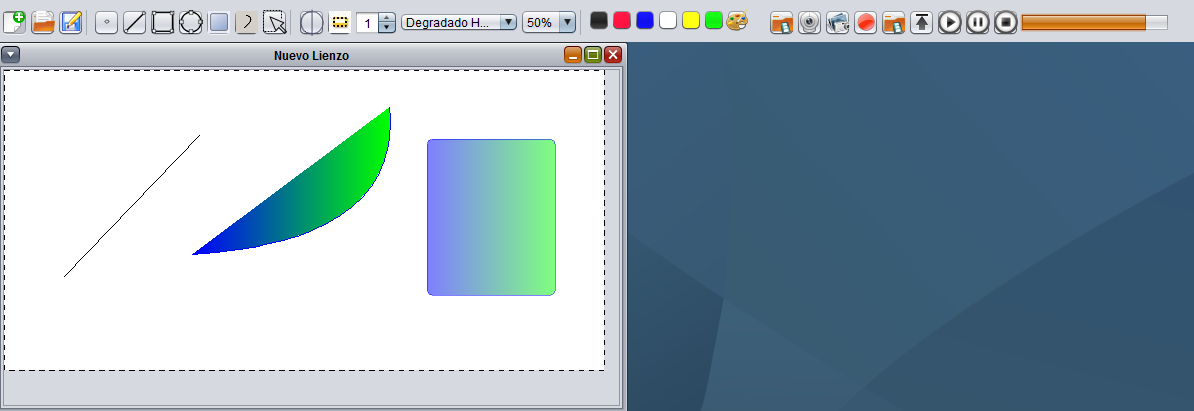
\includegraphics[scale=0.45]{images/barraprogreso}
  \caption{Barra de Progreso 2}
  \label{Barra de Progreso 2}
\end{figure}


\subsection*{Nota:}
Se ha generado tambien \emph{JavaDoc} del proyecto realizado.
%----------------------------------------------------------------------------------------
%clases propias
%funcionalidad botones


\bibliography{citas} %archivo citas.bib que contiene las entradas 
\bibliographystyle{plain} % hay varias formas de citar

\end{document}
